\documentclass[mathpazo]{csam}

\RequirePackage{fix-cm}
% Packages and macros go here
\usepackage{mathrsfs,amsmath,amssymb,bm}
\usepackage{lipsum}
\usepackage{amsfonts}
\usepackage{epstopdf}
\usepackage{makecell, rotating}
\usepackage{multirow}
\usepackage{algorithm} 
\usepackage{algorithmic}
\usepackage{multirow}
\usepackage{subfigure}
\usepackage{xcolor}

\newcommand{\creflastconjunction}{, and~}
\newcommand{\bbR}{\mathbb{R}}
\newcommand{\bbC}{\mathbb{C}}
\newcommand{\bbZ}{\mathbb{Z}}
\newcommand{\bbQ}{\mathbb{Q}}
\newcommand{\bbN}{\mathbb{N}}
\newcommand{\by}{\bm{y}}
\newcommand{\bz}{\bm{z}}
\newcommand{\bx}{\bm{x}}
\newcommand{\tbx}{\tilde{\bm{x}}}
\newcommand{\ba}{\bm{a}}
\newcommand{\bb}{\bm{b}}
\newcommand{\bn}{\bm{n}}
\newcommand{\br}{\bm{r}}
\newcommand{\bh}{\bm{h}}
\newcommand{\bH}{\bm{H}}
\newcommand{\bN}{\bm{N}}
\newcommand{\bk}{\bm{k}}
\newcommand{\bo}{\bm{0}}
\newcommand{\bhphi}{\bm{\hat{\phi}}}
\newcommand{\bhpsi}{\bm{\hat{\psi}}}
\newcommand{\bphi}{\bm{{\phi}}}
\newcommand{\bt}{\bm{t}}
\newcommand{\bs}{\bm{s}}
\newcommand{\bu}{\bm{u}}
\newcommand{\bM}{\bm{M}}
\newcommand{\bP}{\bm{P}}
\newcommand{\bQ}{\bm{Q}}
\newcommand{\bB}{\bm{B}}
\newcommand{\bA}{\bm{A}}
\newcommand{\bI}{\bm{I}}
\newcommand{\calS}{\mathcal{S}}
\newcommand{\calB}{\mathcal{B}}
\newcommand{\calP}{\mathcal{P}}
\newcommand{\calR}{\mathcal{R}}
\newcommand{\calM}{\mathcal{M}}
\newcommand{\calJ}{\mathcal{J}}
\newcommand{\calF}{\mathcal{F}}
\newcommand{\calI}{\mathcal{I}}
\newcommand{\calD}{\mathcal{D}}
\newcommand{\calA}{\mathcal{A}}
\newcommand{\hF}{\hat{F}}
\newcommand{\bq}{\bm{q}}
\newcommand{\hw}{\hat{w}}
\newcommand{\hphi}{\hat{\phi}}
\newcommand{\hPhi}{\hat{\Phi}}
\newcommand{\hpsi}{\hat{\psi}}
\newcommand{\hPsi}{\hat{\Psi}}
\newcommand{\hxi}{\hat{\xi}}
\newcommand{\hJ}{\hat{J}}
\newcommand{\vzero}{\bm{0}}
\newcommand{\tE}{\tilde{E}}
\newcommand{\tF}{\tilde{F}}
\newcommand{\tG}{\tilde{G}}
\newcommand{\tg}{\tilde{g}}
\newcommand{\bg}{\bar{g}}
\newcommand{\tJ}{\tilde{\mathcal{J}}}
\newcommand{\td}{\tilde{d}}
\newcommand{\la}{\langle}
\newcommand{\ra}{\rangle}
\newcommand{\dom}{\mathrm{dom}}
\DeclareMathOperator{\intdom}{\mathrm{int}\dom}
\DeclareMathOperator{\ridom}{\mathrm{ri}\dom}
\DeclareMathOperator{\affdom}{\mathrm{aff}\dom}
\newcommand{\recheck}[1]{{\color{red}{#1}}}



\newcommand\tbbint{{-\mkern -16mu\int}}
\newcommand\tbint{{\mathchar '26\mkern -14mu\int}}
\newcommand\dbbint{{-\mkern -19mu\int}}
\newcommand\dbint{{\mathchar '26\mkern -18mu\int}}
\newcommand\bint{
	{\mathchoice{\dbint}{\tbint}{\tbint}{\tbint}}
}
\newcommand\bbint{
	{\mathchoice{\dbbint}{\tbbint}{\tbbint}{\tbbint}}
}

\allowdisplaybreaks[4]
\DeclareMathOperator*{\argmin}{\mathrm{argmin}}
\DeclareMathOperator*{\argmax}{\mathrm{argmax}}

\newcommand{\Prox}{\mathrm{Prox}}
\newcommand{\BProx}{\mathrm{BProx}}
\newcommand{\GProx}{\mathrm{GProx}}
\newcommand{\dist}{\mathrm{dist}}
%\newcommand{\mod}{\mathrm{mod}}

%\renewcommand{\baselinestretch}{1.5}
\newtheorem{thm}{Theorem}
\newtheorem{assumption}[thm]{Assumption}
% \newtheorem{theorem}{Theorem}[section]
% \newtheorem{lemma}[theorem]{Lemma}

% \theoremstyle{definition}
% \newtheorem{definition}[theorem]{Definition}
% \newtheorem{example}[theorem]{Example}
\newtheorem{xca}[theorem]{Exercise}

\theoremstyle{remark}
% \newtheorem{remark}[theorem]{Remark}


\newcommand{\Note}[1]{{\color{blue}{#1}}} % add by BAO for notice.
\newcommand{\Notsure}[1]{{\color{red}{#1}}} % add by BAO for notice.


%%%%% author macros %%%%%%%%%
% place your own macros HERE
%%%%% end %%%%%%%%%

\begin{document}
	%%%%% title : short title may not be used but TITLE is required.
	% \title{TITLE}
	% \title[short title]{TITLE}
	\title[HiCS]{\textcolor{blue}{A finite-step convergent method 
	of finding a suspected extreme point}}

	%%%%% author(s) :
	
	% multiple authors:
	% Note the use of \affil and \affilnum to link names and addresses.
	% The author for correspondence is marked by \corrauth.
	% use \emails to provide email addresses of authors
	% e.g. below example has 3 authors, first author is also the corresponding
	%      author, author 1 and 3 having the same address.
	\author[Y. Huang and K. Jiang]{
	Yunqing Huang\affil{1}\corrauth~and Kai Jiang\affil{1} }
	\address
	{ \affilnum{1}\ School of Mathematics and Computational Science, 
		Hunan Key Laboratory for Computation and Simulation in Science and Engineering,
		Xiangtan University, Xiangtan, Hunan, 411105, China.}
	\emails{{\tt huangyq@xtu.edu.cn} 
		}
	% \footnote and \thanks are not used in the heading section.
	% Another acknowlegments/support of grants, state in Acknowledgments section
	% \section*{Acknowledgments}
	
	%%%%% Begin Abstract %%%%%%%%%%%
	\begin{abstract}
		{
%\Notsure{
%In our previous work [Adv. Appl. Math. Mech., 2017, 9: 307-323],
%we proposed a novel algorithm, the hill-climbing method with a stick
%(HiCS), to address the unconstrained optimization. 
%HiCS can find a suspected extreme point (SEP) rather than a minimizer. The SEP
%indicates the minimizers exist in a small domain with mild conditions.   
%In this paper, we give a rigorous theory to guarantee that the HiCS has 
%a finite-step convergence property.
%Meanwhile, an efficient discretization strategy based on the regular simplex is
%developed to treat high-dimensional problems. 
%The power of the improved HiCS is demonstrated by several
%high-dimensional benchmarks.
%}
\Note{
Determining a area that contains minimizers is a prerequisite for the
success of optimization methods.  
In our previous work [Adv. Appl. Math. Mech., 2017, 9: 307-323],
we proposed a novel algorithm, the hill-climbing method with a stick
(HiCS), to find a satisfactory domain. 
The HiCS is easy to implement and has only one parameter, the search radius, to be adjusted.
In this paper, we give a rigorously analysis to guarantee that the HiCS converges to 
a suspected minimum point (SMP) within finite steps.
The SMP is a new concept that might be not a minimizer but measures the distance between
the SMP and minimizers being smaller than the search radius.
To address high dimensional problems, we propose an efficient method
to discretize subproblem through simplex and its rotation in which the discretization
points linearly increase with the spatial dimension. We examine the performance of
the HiCS by several high-dimensional benchmarks.  
Numerical results demonstrate that the HiCS can efficiently obtain a
small neighbourhood that contains local minimizers, even the global minimizer.
The obtained results by the HiCS provide a good initial values for other optimization
methods to further find a minimizer. Alternatively, we decrease the search
radius to directly approximate a minimizer by the HiCS.
}
}
	\end{abstract}
	%%%%% end %%%%%%%%%%%
	
	%%%%% AMS/PACs/Keywords %%%%%%%%%%%
	%\pac{}
	\ams{90C56, 90C59, 65K05.%The information of the AMS subject classification can be found in http://mathscinet.ams.org/msc/msc2010.html
	}
	\keywords{
Hill-climbing method with a stick, Suspected minimum point, Finite-step convergence, 
Simplex, High-dimensional problems}
	
	%%%% maketitle %%%%%
	\maketitle
	
\section{Introduction}
\label{sec:intro}

\textcolor{blue}{
Classic optimization approaches are developed to directly find the minimum point}
which can be divided into two
classes, directional search and model-based\,\cite{sun2006optimization,
nocedal2006numerical, conn2009introduction}.  Directional search algorithms first
determine the search direction and then the step length along with the search
direction. Model-based approaches construct and utilize a related simple model to
approximate the original problem in a trust region to guide the search process. 
\textcolor{blue}{
Before finding a minimizer, a prerequisite is 
determining that there exist minimizers in the search domain.
}
Inspired by the behavior of the blind for climbing hill, we
proposed a new approach, the HiCS, to \textcolor{blue}{greatly shrink the search
domain which includes minimizers}\,\cite{huang2017hill}.
The main idea of the HiCS, at each search step, is comparing
function values on a surface surrounding the current iterator.
It requires a comparison of function values, and does not need the search direction
or construct a surrogate model in a trust region.
\textcolor{blue}{
The HiCS is different from the direct search methods in
derivative-free optimization\,\cite{kolda2003optimization, conn2009introduction}. The
direct search methods choose a set of nonzero vectors deterministically or
stochastically as search directions, then try to find a replaceable point along
search directions with a step size until a certain stopping criterion is met.  The
HiCS finds a neighbourhood that contains minimum points rather than directly finding them. 
}
Numerical results have been demonstrated that the HiCS has many 
satisfactory properties, including being easy to implement,
a unique parameter to be modulated, and having the capacity
of \textcolor{blue}{finding a small domain of the local and global minimizer. }
However, there are two unsolved problems in the
previous work, including a rigorous theoretical explanation and
the treatment of high-dimensional problems.
This paper will give the convergence analysis and related
properties of this algorithm by introducing a new concept, the suspected extreme
point.
Meanwhile, a new strategy will be proposed to discretize the search
surface for high-dimensional objective functions.

In the following, we will briefly introduce the HiCS and
prove its finite-step convergence in Sec.\,\ref{sec:algorithm}. 
The algorithm implementation is presented in Sec.\,\ref{sec:implement}.
In particular, the new sampling strategy using the regular simplex is
also given in this section.
The numerical experiments including high-dimensional benchmarks
are showcased in Sec.\,\ref{sec:experiment}. 
Finally the conclusion and discussions are given in Sec.\,\ref{sec:conclusion}.

\section{HiCS and convergence analysis}
\label{sec:algorithm}

Before going further, a short introduction of the HiCS is necessary.
We consider an unconstrained optimization problem 
\begin{align}
	\min_{x\in\Omega\subset\mathbb{R}^d} f(x),
	\label{}
\end{align}
where the objective function $f(x):\bbR^d\rightarrow \bbR$.
Let $\rho$ be the search radius, $O(x_k, \rho)=\{x:
\|x-x_k \|=\rho\}$ be the search surface at the
$k$-th iteration with radius $\rho$. $\|\cdot \|$ is the common
norm in $\bbR^d$ space. Denote $U(x_k, \rho)$ is the neighbourhood of
$x_k$ with radius of $\rho$.  
$\overline{U}(\tilde{x}, \rho)$ is the closure of $U(\tilde{x}, \rho)$, i.e., 
$\overline{U}(\tilde{x}, \rho) = U(\tilde{x}, \rho)\cup O(\tilde{x}, \rho) $.
To illustrate the algorithm more accurately, an useful concept of the
\textit{suspected extreme point} is proposed.

\textcolor{blue}{
\begin{definition}	
	For a given objective function $f(x)$ and a positive constant 
	$\rho>0$, $\tilde{x}$ is a \textit{suspected extreme point} if
	$f(\tilde x)\leq f(x)$ or $f(\tilde x)\geq f(x)$, for each $x \in O(\tilde{x},\rho)$.
	If $f(\tilde x) \leq f(x)$ for all $x\in O(\tilde{x},\rho)$,
	$\tilde{x}$ is the \textit{suspected minimum point (SMP)}.
\end{definition}
\begin{remark}
	Note that the SMP might be not a minimizer. If the SMP is found which means
	that the minimizer point is close to it.
	If $f(x)$ is continuous in $\overline{U}(\tilde{x}, \rho)$,
	$\tilde x$ is a SMP, then there exists at least a minimizer in $U(\tilde x,
	\rho)$ or $f(x)$ is constant on $\overline{U}(\tilde x, \rho)$.
\end{remark}
}


%Obviously, $\tilde{x}$ is a SMP if $\tilde{x}$ is a minimizer in
%the neighborhood of $U(\tilde{x}, \rho)$. The opposite is not always true.
With these notations, the HiCS can be presented
as the Algorithm \ref{alg:HiCS}.
\begin{algorithm}[H]
	\caption{Hill-Climbing method with a stick (HiCS)}
	\label{alg:HiCS}
\begin{algorithmic}[1]
	\STATE \textbf{Initialization:} Choose $x_0$ and $\rho$.
	\STATE \textbf{For} $k=0,1,2,\dots$
	\STATE \hspace{0.5cm} 
	\textcolor{blue}{Find $\bar{x}=\argmin_{x\in O(x_k,~ \rho)} f(x)$. }
			\\
	\STATE \hspace{0.5cm} If $f(\bar x)<f(x_k)$, then set $x_{k+1}= \bar{x}$.
		  \\
	\STATE \hspace{0.5cm} Otherwise, declare that 
		   a SMP is found, and end the iteration.
\end{algorithmic}
\end{algorithm}
\textcolor{blue}{ 
In what follows, we will discuss the convergent property of the Algorithm
\ref{alg:HiCS}.
}
\begin{theorem}[Finite-step convergence]
	\label{thm:fsc}
	Suppose that the objective function $f(x)$ is continuous and the
	search domain $\Omega$ is a compact set.
	If there are not two SMPs $x_*$ and $x^*$ satisfying 
	$\|x_*-x^*\|=\rho$ and $f(x^*)=f(x_*)$.
	Then Algorithm \ref{alg:HiCS} converges in finite steps.
\end{theorem}
\begin{proof}
	Assume that the HiCS generates an infinite pair sequence
	$\{x_n, f(x_n)\}_{x=0}^{\infty}$. From these assumptions,
	it is obvious $f(x)$ is bounded. The decreasing sequence
	$\{f(x_n)\}_{n=0}^\infty$ converges, and the bounded
	$\{x_n\}_{n=0}^\infty$ has a convergent subsequence 
	$\{x_{n_k}\}_{k=0}^\infty$. Assume that $f(x_n)\rightarrow
	\alpha$ and $x_{n_k}\rightarrow x^*$. Obviously $x^*$ is a SMP.
	
	According to the subsequence
	$\{x_{n_k}\}_{k=0}^\infty$, we can always choose an another
	bounded subsequence $\{x_{n_k -1}\}_{k=0}^\infty \subset
	\{x_n\}$ satisfying $\|x_{n_k - 1}-x_{n_k}\|=\rho$. 
	Due to the boundedness of iteration
	sequence, $\{x_{n_k-1}\}_{k=0}^\infty$ has a convergent
	subsequence $\{x_{n_{m}}\}_{m=0}^\infty$. Let $x_{n_m}
	\rightarrow x_*$ when $m\rightarrow \infty$. $x_*$ is also a SMP.
	From the $\{x_{n_m}\}$, we can find a subsequence
	$\{x_{n_{m}+1}\}\subset \{x_{n_k}\}$ which satisfies
	$\|x_{n_m}-x_{n_{m}+1}\|=\rho$, and $x_{n_{m}+1}\rightarrow x^*$
	($m\rightarrow \infty$).
	Obviously, $\|x^*-x_*\|=\rho$, and $f(x^*)=f(x_*)=\alpha$ 
	which clearly contradicts the assumption.
\end{proof}
\textcolor{blue}{ 
Theorem \ref{thm:fsc} demonstrates that the HiCS can converge to a SMP $x_k$ in finite
steps under reasonable conditions. If the stopping criterion is met, it implies
that there exist minimizers in $U(x_k, \rho)$. The distance between the SMP
$x^k$ and minimizers is smaller than $\rho$.
Therefore, the HiCS can efficiently shrink search domain $\Omega$ to the $U(x_k,
\rho)$.  At each iteration, the HiCS minimizes a
$(d-1)$-dimensional subproblem of the $d$-dimensional objective function.
In practice, HiCS requires to numerically solve the subproblem
in the Algorithm \ref{alg:HiCS}.
Next, we will discuss the implementation in detail. 
}

%The approximation error of the HiCS can be measured by the distance between the
%SMP and a minimum.  When the HiCS converges, the approximation error is smaller
%than the search radius $\rho$.
%From our experience, the HiCS usually terminates in finite steps. It is a
%satisfactory property. In what follows, we will
%prove the finite-step convergence with some mild conditions.



\section{Implementation}
\label{sec:implement}

\textcolor{blue}{ 
As mentioned above, at each iteration, the HiCS has to discretize 
the $(d-1)$-dimensional search surface $O(x_k,\rho)$
to numerically imitate the minimization process of finding $\tilde{x}$.
How to design an efficient method to discretize $O(x_k,\rho)$ is skillful. 
}
When without a priori information of the objective function, the discretization
principles for $O(x_k,\rho)$ should include symmetric and uniform distribution
and as few discretization points as possible.
Previous results have shown that the uniformly distributed
discretization method based on the spherical coordinate
can be used to find the SMP\,\cite{huang2017hill}. 
The generated discretization points are as large as \textcolor{blue}{$2^{d}m$} in
each iteration, $m$ is the number of refinement, $d$ is the dimension of
the objective problem. 
\textcolor{blue}{ 
The exponential growth of discretization points with the spatial dimension $d$
restricts the application to high-dimensional problems. 
}
To overcome this limitation, it needs to develop a new
strategy to discretize the search surface $O(x_k,\rho)$ with fewer
discretization points but still satisfying these properties.
A reasonable requirement for discretization points should be
linear or quasi-linear growth as the dimension of the objective problem increases.
In this work, we will use the regular simplex and its rotations to
discretize $O(x_k,\rho)$. 
The computational complexity grows linearly as $d$ increases.

The $d$-dimensional regular simplex is a congruent polytope of
$\mathbb{R}^d$ with a set of points $\{a_1,\dots,a_d,a_{d+1}\}$,
and all pairwise distances $1$.
Its Cartesian coordinates can be obtained from the following two properties:
\begin{enumerate}
	\item For a regular simplex, the distances of its vertices 
		$\{a_1,\dots,a_d,a_{d+1}\}$ to its center are equal.
	\item The angle subtended by any two vertices of the 
		$d$-dimension simplex through its center is
		$\arccos(-1/d)$.
\end{enumerate}
In particular, the above two properties can be implemented
through the Algorithm \ref{alg:simplex}.
\begin{algorithm}[!htpb]
	\caption{Generate $d$-D regular simplex coordinates} 
	\label{alg:simplex}
\begin{algorithmic}
	\STATE Given a $d\times(d+1)$-order zero matrix $x(1:d,1:d+1)$
	\STATE Let $x(:,1) = (1,0,\dots,0)$
	\FOR {$i=2:1:d$}
	\STATE $x(i,i)=\sqrt{1-\sum_{k=1}^{i-1} [x(k, i)]^{2}}$
		\FOR {$j=i+1:1:d+1$}
		\STATE $x(i,j)
		=-\dfrac{1}{x(i,i)}\Big[\dfrac{1}{d}+x(1:i-1, i)^T \cdot
		x(1:i-1, j\,)\Big]$
		\ENDFOR
	\ENDFOR
	\STATE Output the column vectors, and let $a_j=x(:,j)$,
	$j=1,2,\dots,d+1$ 
\end{algorithmic}
\end{algorithm}

If the HiCS does not find a better state at the initial given regular simplex,
more points can be added to discretize $O(x_k, \rho)$ by rotating regular
simplex. For a given rotation angle $\theta=(\theta_1,\theta_2,\dots,\theta_{d})$, 
the rotation matrix $\bm Q$ is given as 
\begin{equation}
\begin{aligned}
	{\bm Q} = 
	 \prod_{i=2}^{d-1} &
\bordermatrix{
  &  &       &  & 		   & i &		   &  &  & \cr
  & 1&       &  & 		   & \vdots  & 		   &  &  &  \cr
  &  & \ddots&  & 		   & \vdots  & 		   &  &  &  \cr
  &  &       & 1&          & \vdots  & 		   &  &  &  \cr
  &  &       &  & \cos \theta_i & 0 & -\sin \theta_i &  &  &  \cr
  &  &       &  &   0	 & 1 &     0     &  &  & \cr 
  &  &       &  & \sin \theta_i & 0 &  \cos \theta_i &  &  &  \cr
  &  &       &  &          &   &           & 1 & &  \cr
  &  &       &  &          &   &           &  & \ddots &   \cr
  &  &       &  &          &   &           &  &  & 1 
}
\\
	& \begin{pmatrix}
  \cos \theta_1 & -\sin \theta_1 & 0 &  		&   \\
  \sin \theta_1 & \cos \theta_1  & 0 & 	 	& 	\\
  	0	   &      0    & 1 & 		&   \\
  		   & 		   &   & \ddots &   \\
  		   & 		   &   &   		& 1 
	\end{pmatrix}
	\begin{pmatrix}
  1 &  &  &  		&   \\
    & \ddots  &  & 	 	& 	\\
    &    & 1 & 	0	& 0  \\
    &    & 0 & \cos\theta_d & -\sin\theta_d  \\
    & 	 & 0 &  \sin\theta_d & \cos\theta_d 
	\end{pmatrix}.
\end{aligned}
	\label{}
\end{equation}
Then vertices of new simplex are
\begin{align}
	a_j = \bm{Q}a_j + x_k, \quad j = 1,\dots, d+1.
	\label{}
\end{align}
\begin{figure}[!htbp]
	\centering
	\subfigure[Two-dimensional regular simplexes with rotation]{
%      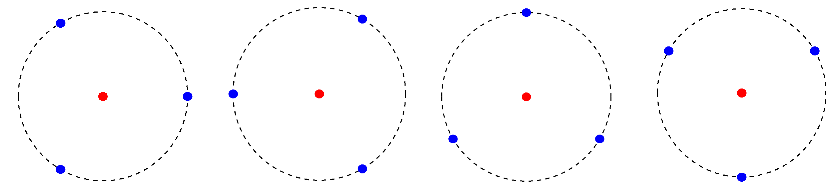
\includegraphics[scale=0.3]{../figures/2Dsketch.png}
		  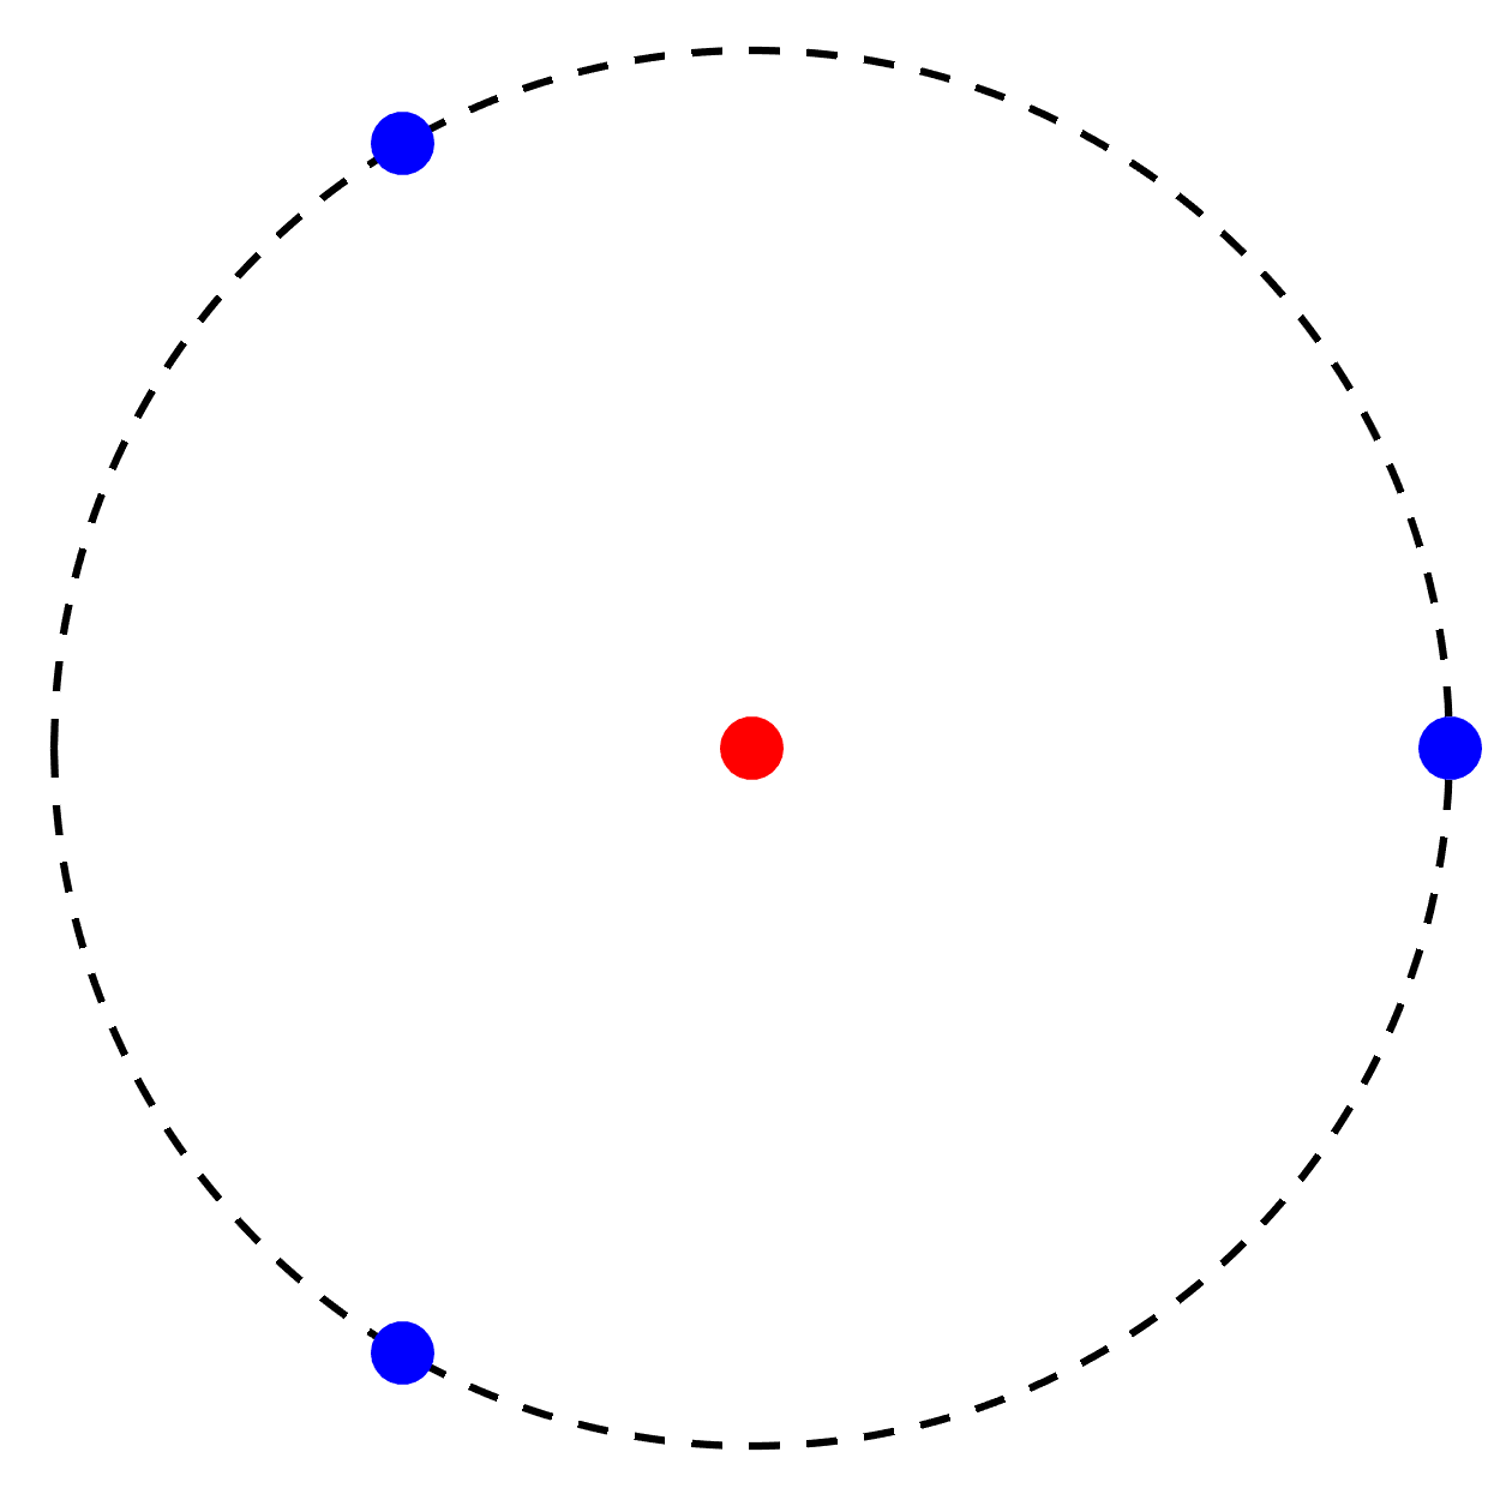
\includegraphics[scale=0.1]{../figures/2D1.png}
		  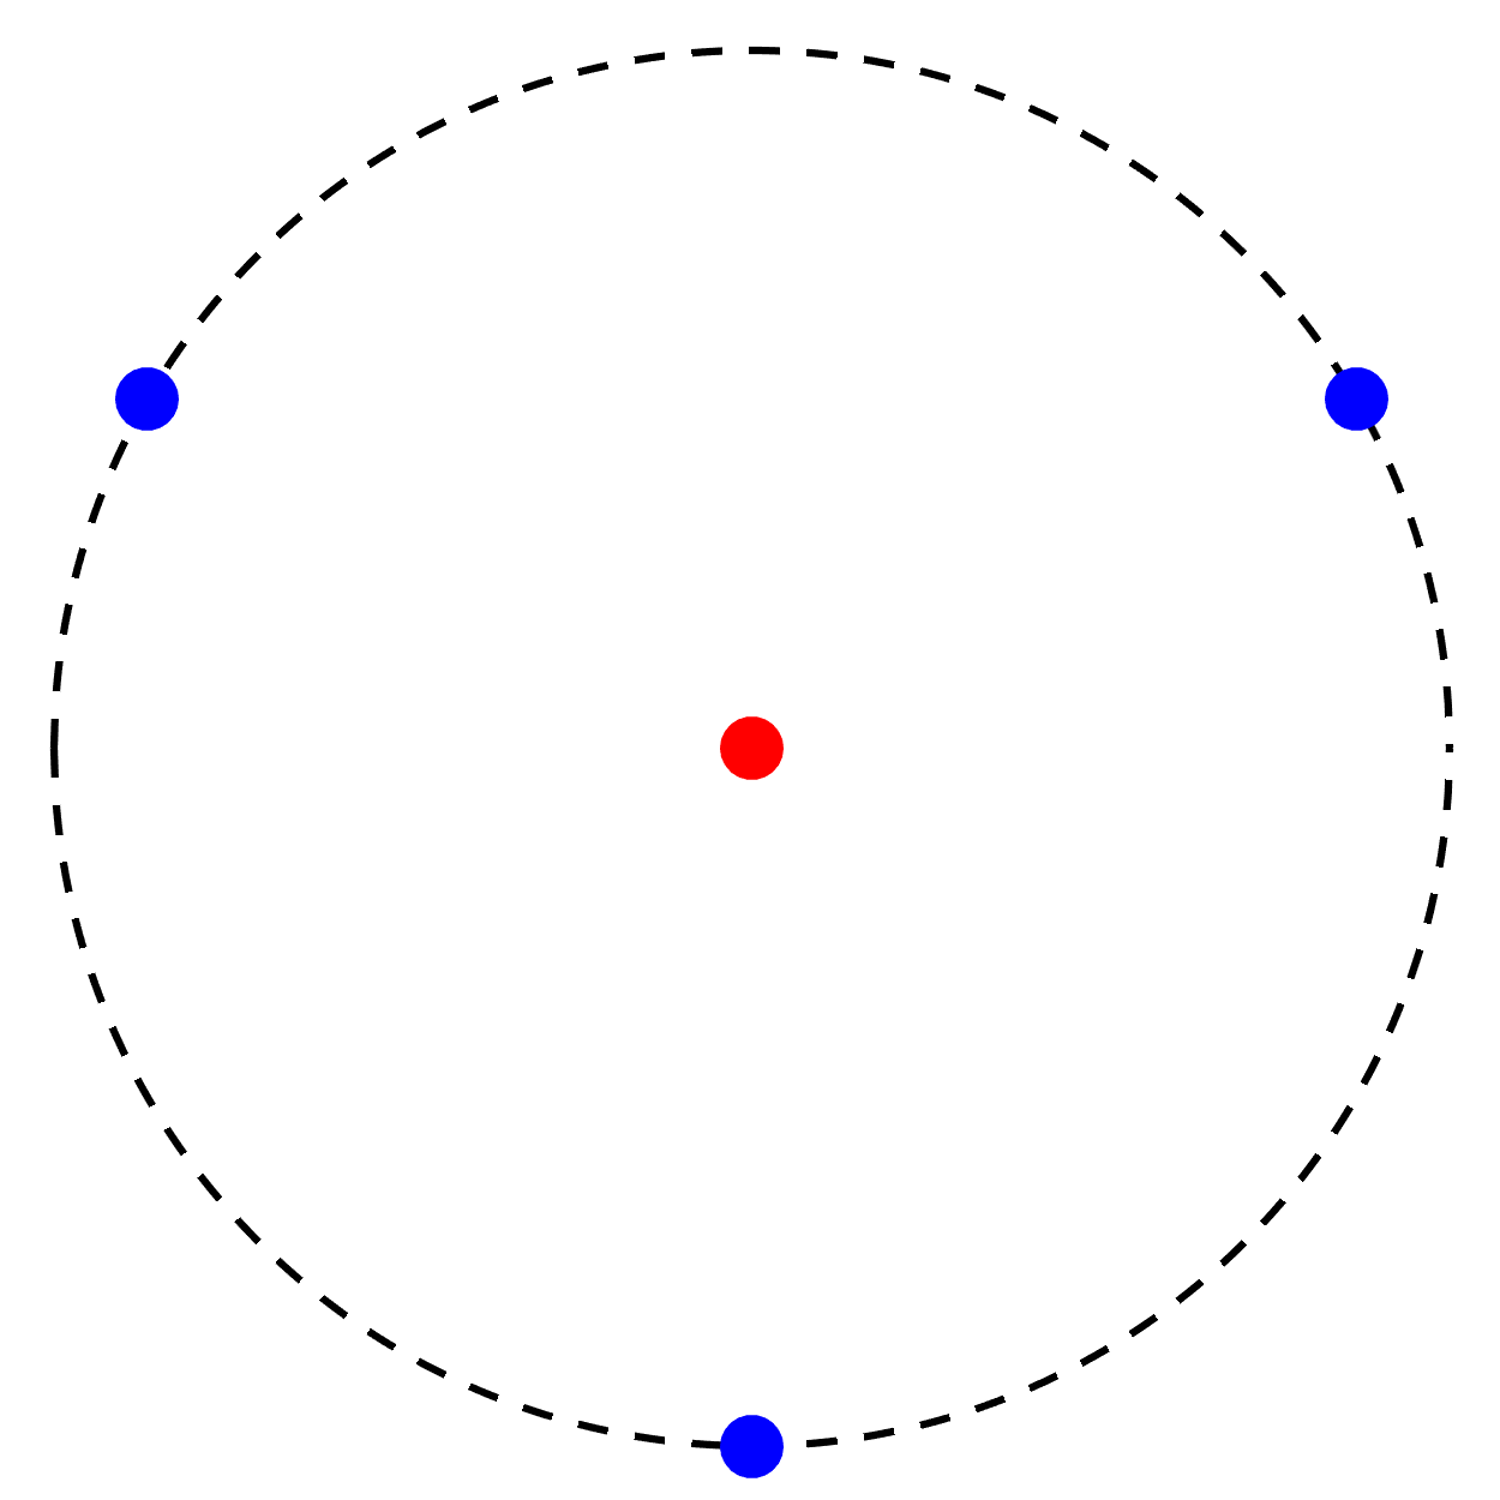
\includegraphics[scale=0.1]{../figures/2D2.png}
		  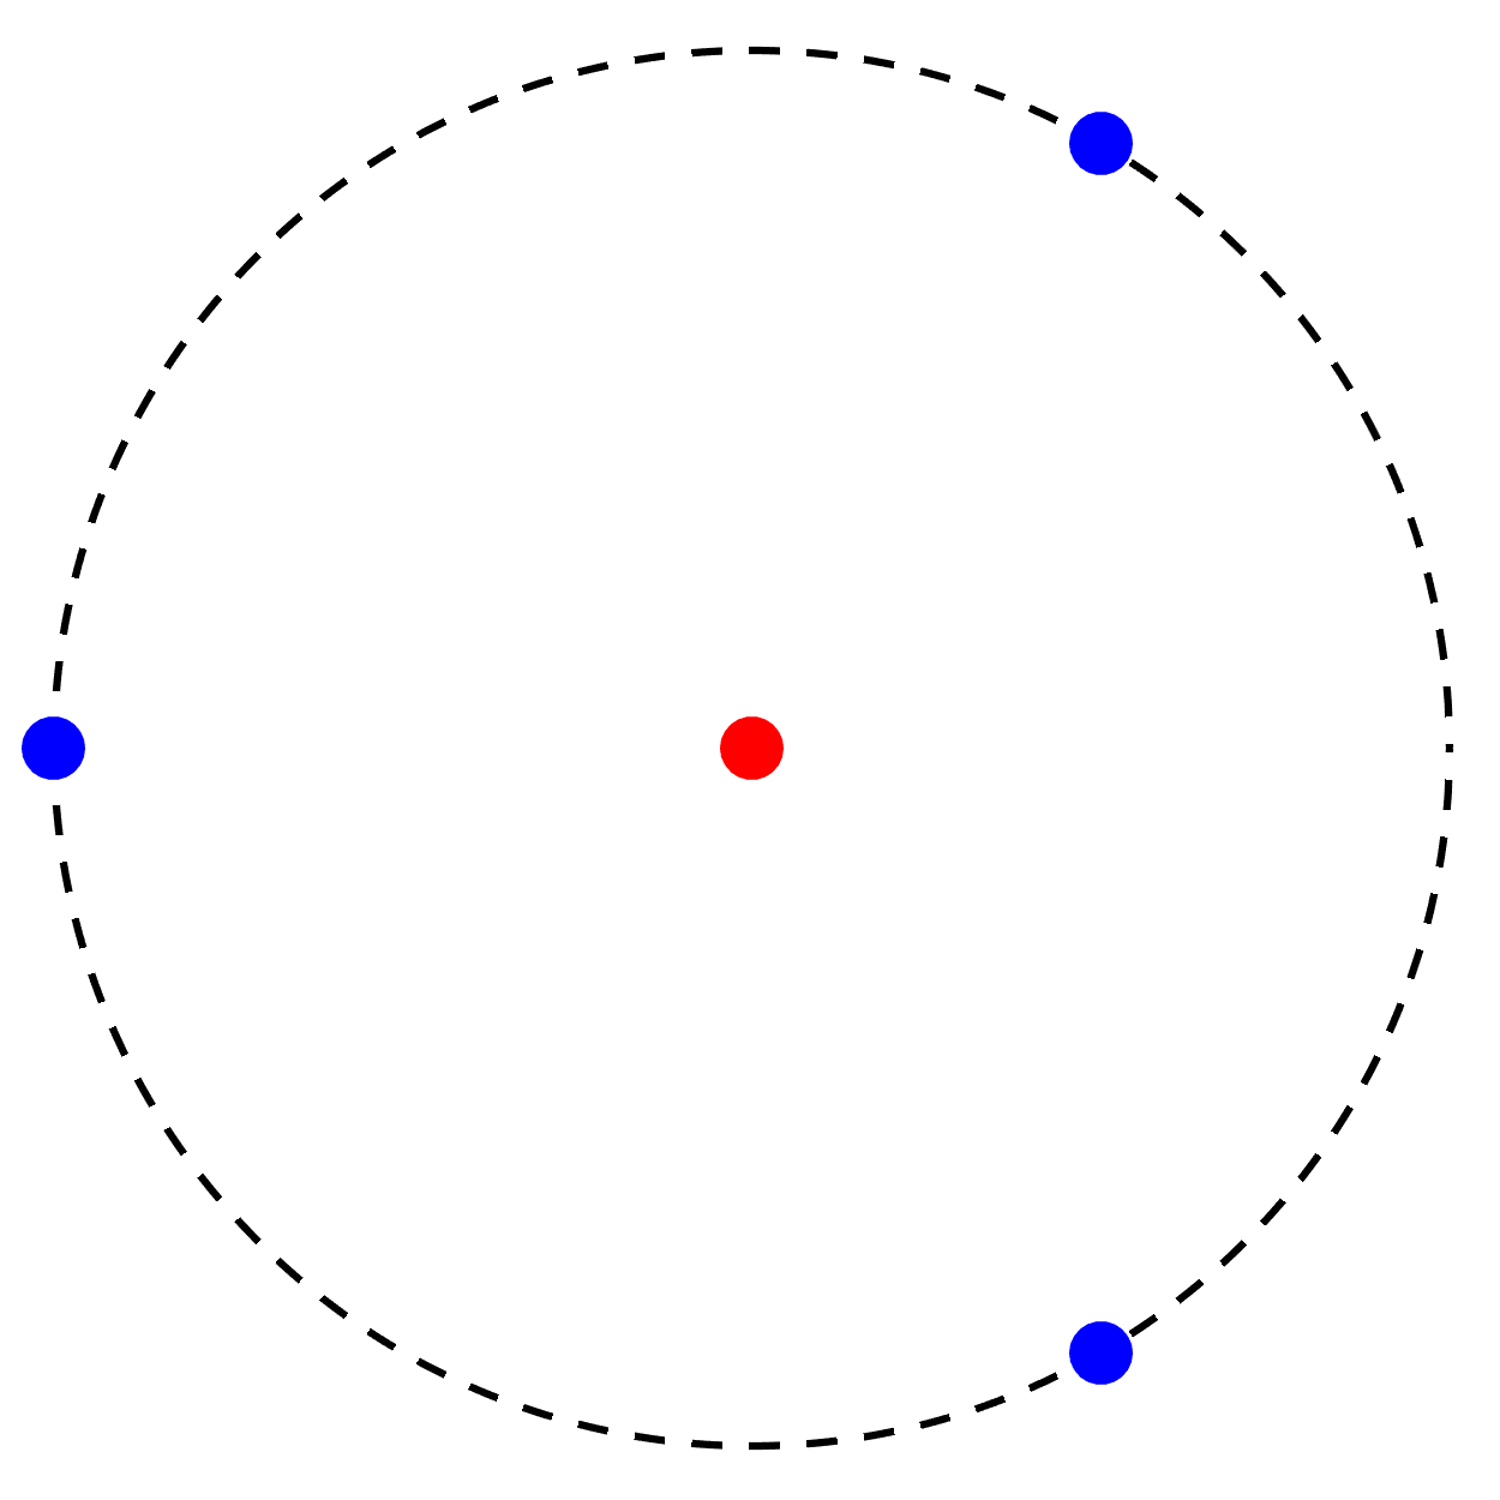
\includegraphics[scale=0.1]{../figures/2D3.png}
		  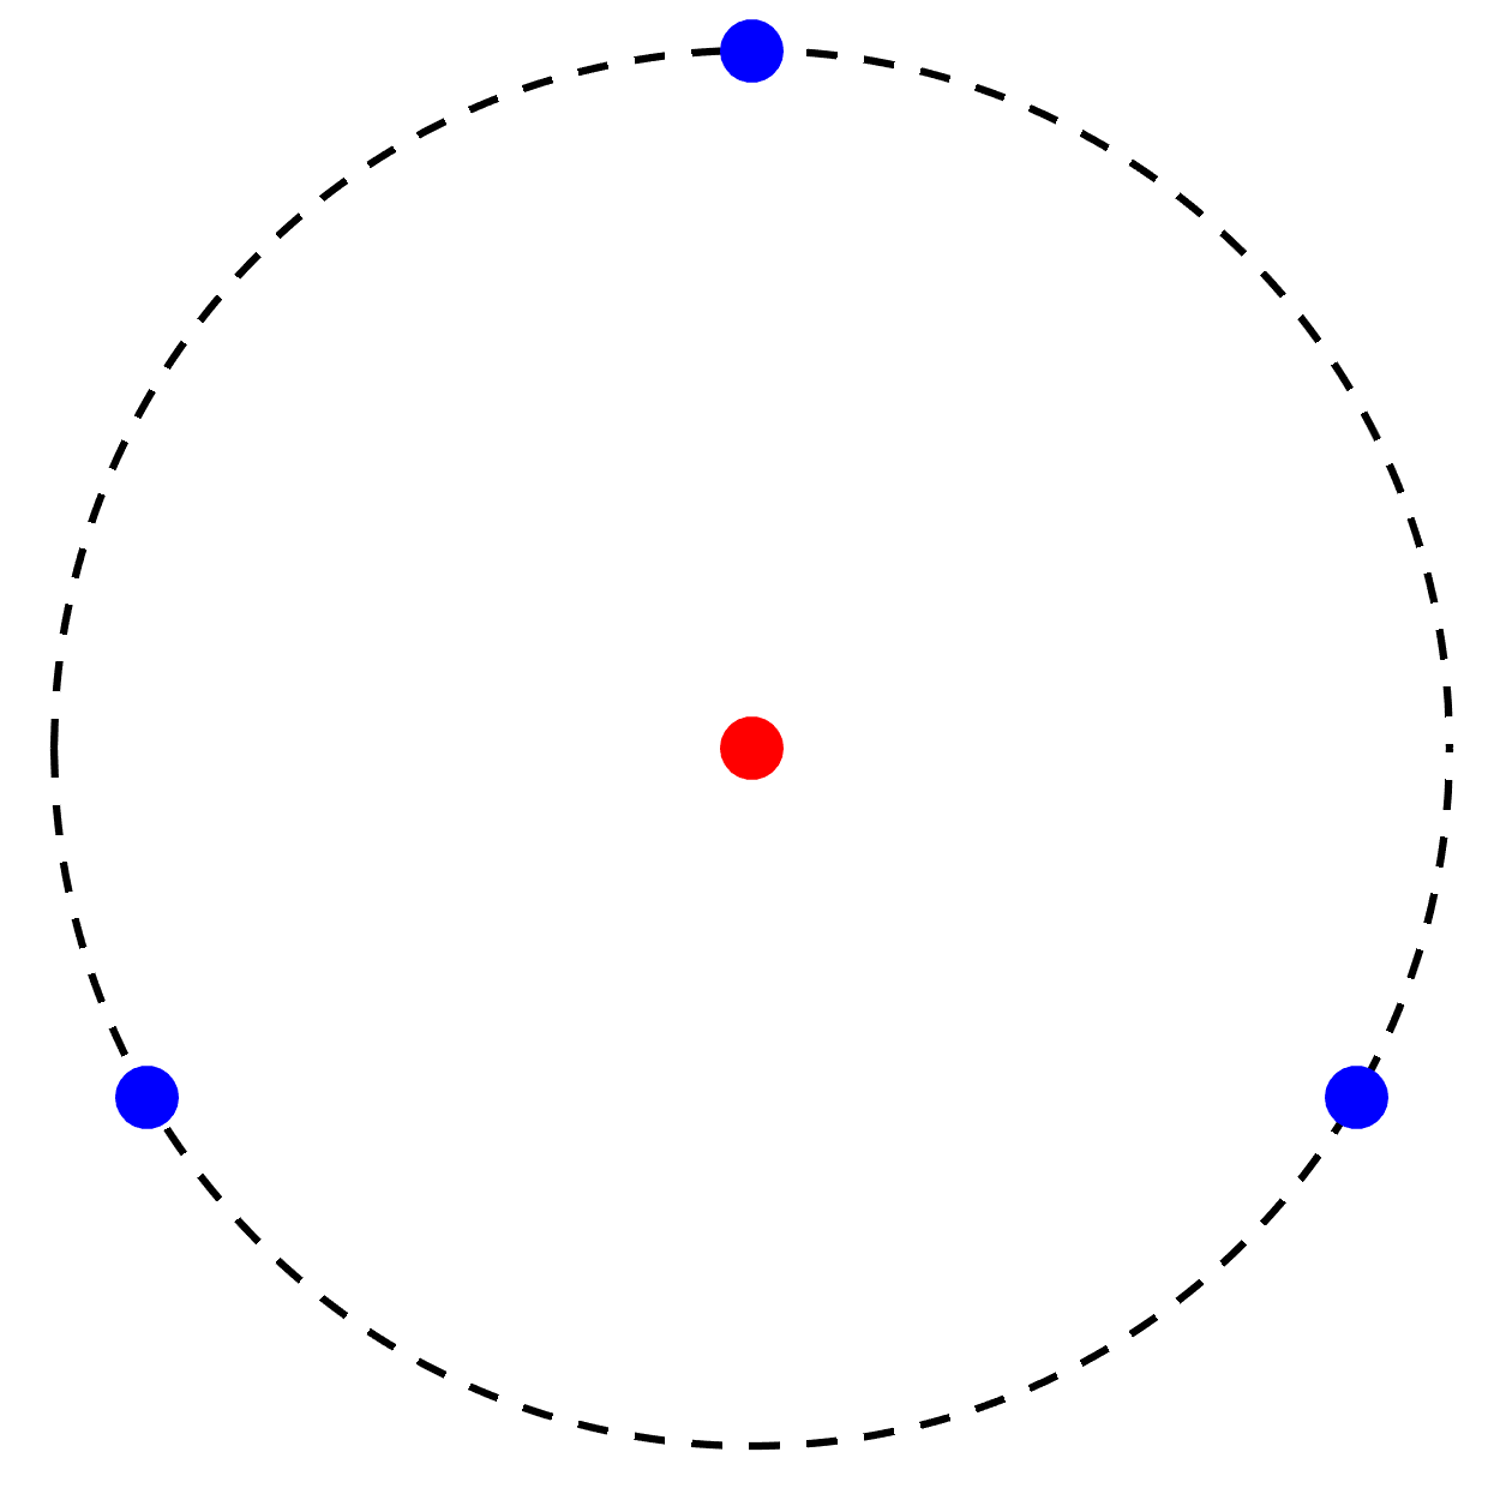
\includegraphics[scale=0.1]{../figures/2D4.png}
	  }
	\subfigure[Three-dimensional regular simplexes with rotation]{
	  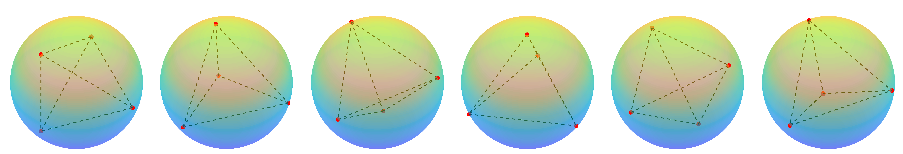
\includegraphics[scale=0.46]{../figures/3Dsketch.png}
	  }
	\caption{The regular simplexes of discretizing the search set $O(x_k, \rho)$
	which obeys uniform distribution principle.}
\label{fig:obset:sketch}
\end{figure}
\textcolor{blue}{
Standard two- and three-dimensional rotational simplexes which obey the uniform
distribution principle are shown in Fig.\,\ref{fig:obset:sketch}.
It should be noted that there could be other strategies to discretize
$O(x_k,\rho)$ if more information is considered. 
For example, the new adding discretized points can be concentrated on these
areas that the function values have a sufficient decrease.
}

To further save computational amount, we choose a dynamic refinement
strategy to discretize the search surface and minimize the subproblem 
in practical implementation.
\Note{
These simplexes satisfies the uniform distribution principle.
}
Based on the dynamic refinement strategy, we propose the
practical HiCS, as the Algorithm \ref{alg:refined} shows.
For a given search radius $\rho$, the computational
amount of the HiCS is not larger than $(d+1)m_{\max}$ in each iteration, 
$m_{\max}$ is the maximum number of rotation,
which is linearly dependent on the spatial dimension $d$.
Therefore, this strategy can allow us to treat high-dimensional optimization
problems due to the economical computational cost.

\begin{algorithm}[!hbpt]
	\caption{Practical HiCS}
	\label{alg:refined}
\begin{algorithmic}[1]
	\STATE Input $x_0$, $\rho>0$, and $m_{\max}\in \mathbb{Z}^+$
	\FOR {$k=0,1,2,\cdots$}
		\STATE Set $m=0$
		\IF {$m\leq m_{\max}$}
			\STATE Discretize $O(x_k,\rho)$ to obtain $O^m_h(x_k,\rho)$. 
			\textcolor{blue}{ Find $x_j=\argmin_{x\in O^m_h(x_k,\rho)} f(x)	$. }
			\IF { $f(x_j)<f(x_k)$}
				\STATE Set $x_{k+1}=x_j$, and $m=m_{\max}+1$
			\ELSE
				\STATE Set $m = m+1$
			\ENDIF
		\ELSE
			\STATE Declare that find a SMP, end program
		\ENDIF
	\ENDFOR
\end{algorithmic}
\end{algorithm}

It is evident that once the HiCS converges, the search space shrinks to a
neighborhood of the SMP with the radius $\rho$, and more significantly, the
convergent neighborhood contains minimizers. 
We will demonstrate this by several numerical experiments in
Sec.\,\ref{sec:experiment}. Note that the convergent result also provides a good
initial value for other optimization approaches, including directional search
and model-based algorithms.  
\Note{We can also modify the HiCS to find a minimizer by changing the search
radius $\rho$ as the Algorithm\,\ref{alg:AHiCS} shows.
In the Algorithm\,\ref{alg:AHiCS}, we can decrease the search radius $\rho$ by
setting $\rho=\eta\rho$ ($\eta<1$), if a SMP
is found for a fixed $\rho$. A small $\rho$ also shortens 
the distance between the SMP and a minimizer. As $\rho$ goes to $0$, the SMP might
become a minimizer.
Certainly, the search surface can be expanded by setting the regulator
$\eta>1$ if required.  The Algorithm\,\ref{alg:AHiCS} can be restarted by fixed
$k$ iterations or by other criterions with different search radius.
}

\begin{algorithm}[H]
	\caption{Adaptive HiCS}
	\label{alg:AHiCS}
\begin{algorithmic}[1]
	\STATE Input $x_0$, $\rho$, $\varepsilon$ and $\eta>0$ and $m_{\max}\in \mathbb{Z}^+$
	\IF {$\rho>\varepsilon$}
	\STATE Carry out the practice HiCS method (see the Algorithm \ref{alg:refined})
		\IF {a SMP is found}
			\STATE Set $\rho=\eta \rho$
		\ENDIF
\ENDIF
\end{algorithmic}
\end{algorithm}

%\begin{algorithm}[H]
%    \caption{Adaptive HiCS}
%    \label{alg:AHiCS}
%\begin{algorithmic}[1]
%    \STATE Input $x_0$, $\rho$, 
%    $\varepsilon$ and $\eta>0$ and  $m_{\max}\in \mathbb{Z}^+$
%    \IF {  $\rho>\varepsilon$}
%    \FOR {$k=0,1,2,\cdots$}
%        \STATE Set $m=0$
%        \IF {$m\leq m_{\max}$}
%            \STATE Discretize $O(x_k,\rho)$ to obtain $O^m_h(x_k,\rho)$
%            \IF {$\exists x_j \in O^m_h(x_k,\rho)$, s.t.  $f(x_j)<f(x_k)$}
%            \STATE Set $x_{k+1}=x_j$, 
%                and $m=m_{\max}+1$
%            \ELSE
%                \STATE Set $m = m+1$
%            \ENDIF
%        \ELSE
%            \STATE Set $\rho=\eta\rho$
%        \ENDIF
%        \STATE Set $k=k+1$
%    \ENDFOR
%\ENDIF
%\end{algorithmic}
%\end{algorithm}


\section{Numerical results}
\label{sec:experiment}

In this section, we choose two kinds of high-dimensional optimization functions,
including the unimodal Gaussian function, multimodal problems, to demonstrate
the performance of the HiCS.
These objective functions are all differentiable. However, it is
emphasized that the HiCS can be applied to non-differentiable problems. 
In Algorithm\,\ref{alg:refined}, the discretized points of 
search set in each iteration are $m(n+1)$, $n$ is the dimension
of objective function. If not specified, the maximum number of
rotation $m=32$.

\subsection{The unimodal problem: Gaussian function}
\label{subsec:gauss}

The first objective function is the unimodal Gaussian problem
\begin{align}
	f(x) = -20\exp\left(-\sum_{j=1}^d x_j^2 \right),
	\label{eqn:exp1}
\end{align}
which a unique minimizer $0$ with $f(0)=-20$.
The objective function is differentiable in $\bbR^d$, however,
it quickly diffuses out towards zero out of the upside-down ``bell''. 

We first investigate the convergent property of HiCS
for $10$ dimensional Gaussian function using 
$30$ experiments.
In the set of experiments, the search radius $\rho$ is fixed as
$0.3$, start points are all randomly generated in the space $[-1,
1]^{10}$.  For each experiment, the HiCS indeed converges and
captures a neighborhood of the peak
$0$ in finite iterations as the Theorem \ref{thm:fsc} predicts.
The Fig.\,\ref{fig:gauss} gives the required iterations for
convergence in $30$ numerical experiments.
\begin{figure}[t]
	\centering
	  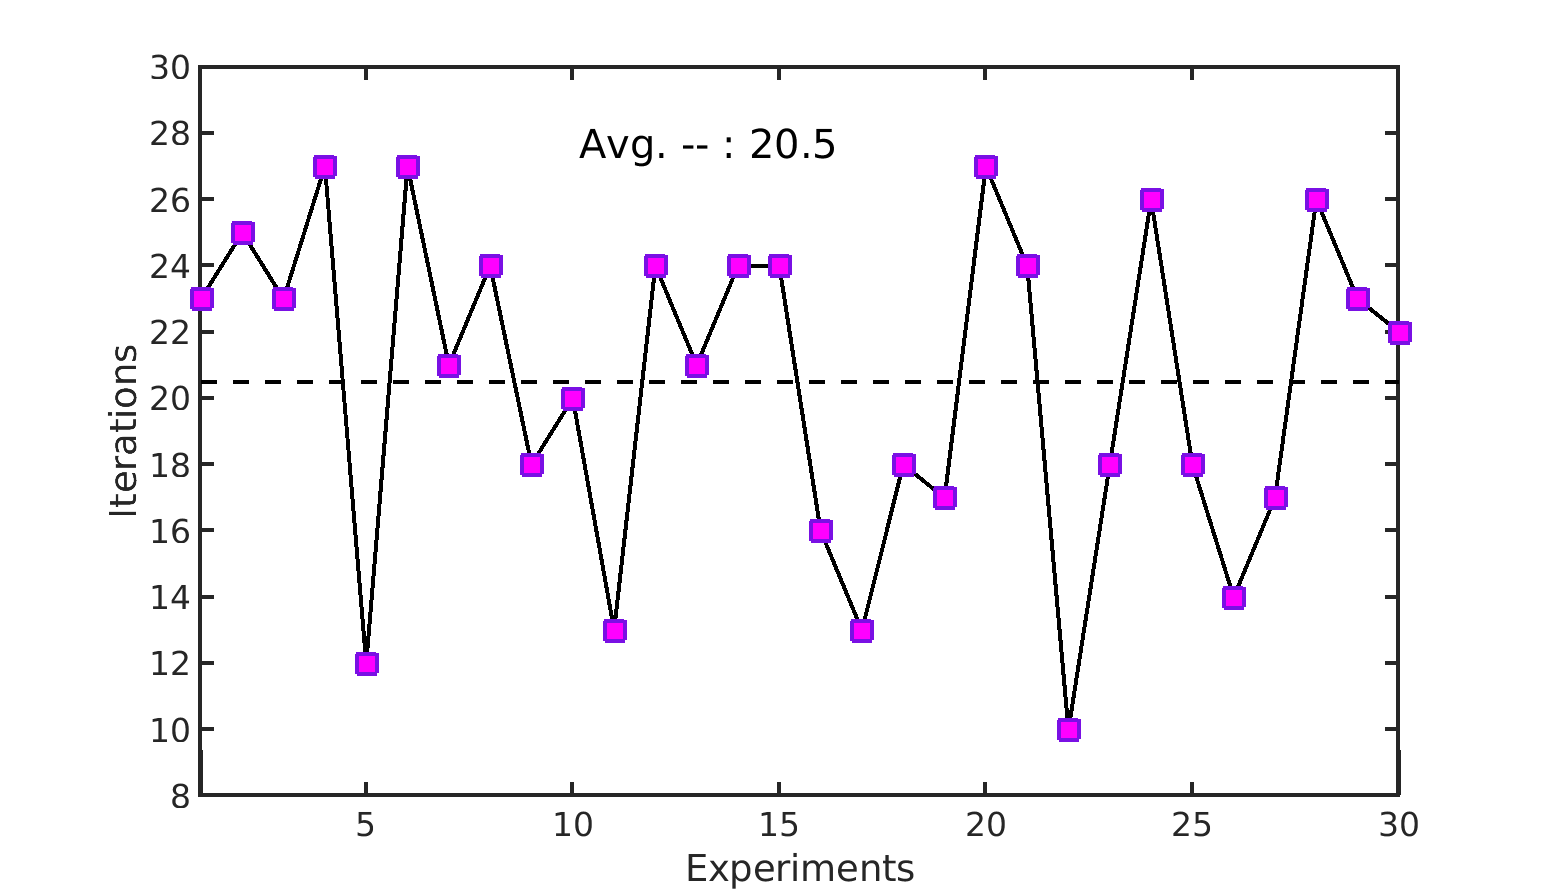
\includegraphics[scale=0.2]{../figures/gauss10Drandr0_3.png}
	  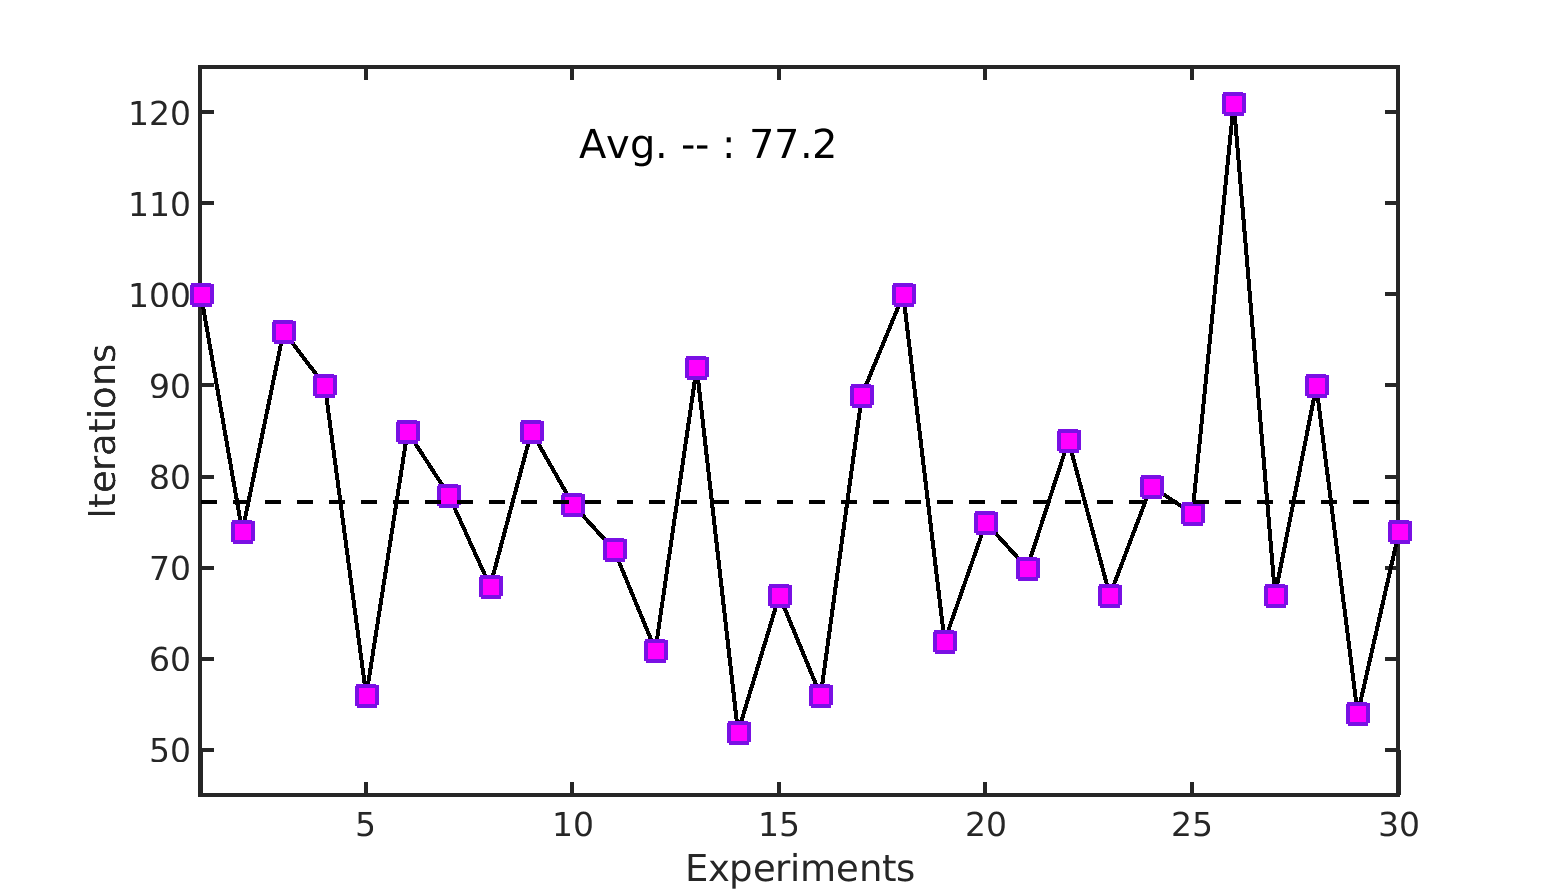
\includegraphics[scale=0.2]{../figures/gauss10Drandr0_1.png}
	  \caption{
	  The required iteration steps of the 
	  HiCS for the Gaussian function
	  \eqref{eqn:exp1} in $30$ runs with randomly generated start points
	  in the space $[-1, 1]^{10}$, and (\textbf{Up}) $\rho=0.3$, (\textbf{Down})
	  $\rho=0.1$. The flat dashed line shows the average.} 
	  \label{fig:gauss}
\end{figure}
In these $30$ runs, the average iterations of convergence is
$20.5$, while the maximum is $27$, and the minimum is $9$.

Then we decrease the search radius $\rho$ to $0.1$ to observe the behavior of
HiCS in $30$ numerical tests. 
The initial values are also randomly generated in the same region.  
The required iterations for convergence are given in the
Fig.\,\ref{fig:gauss}.
In these $30$ runs, the average iterations of convergence are
$77.2$, while the maximum is $121$, and the minimum is $54$.
From these results, the HiCS converges in
finite iterations. Meanwhile, it is obvious that the value of
$\rho$ affects the number of iterations. 
%\begin{figure}[!htbp]
%    \centering
%      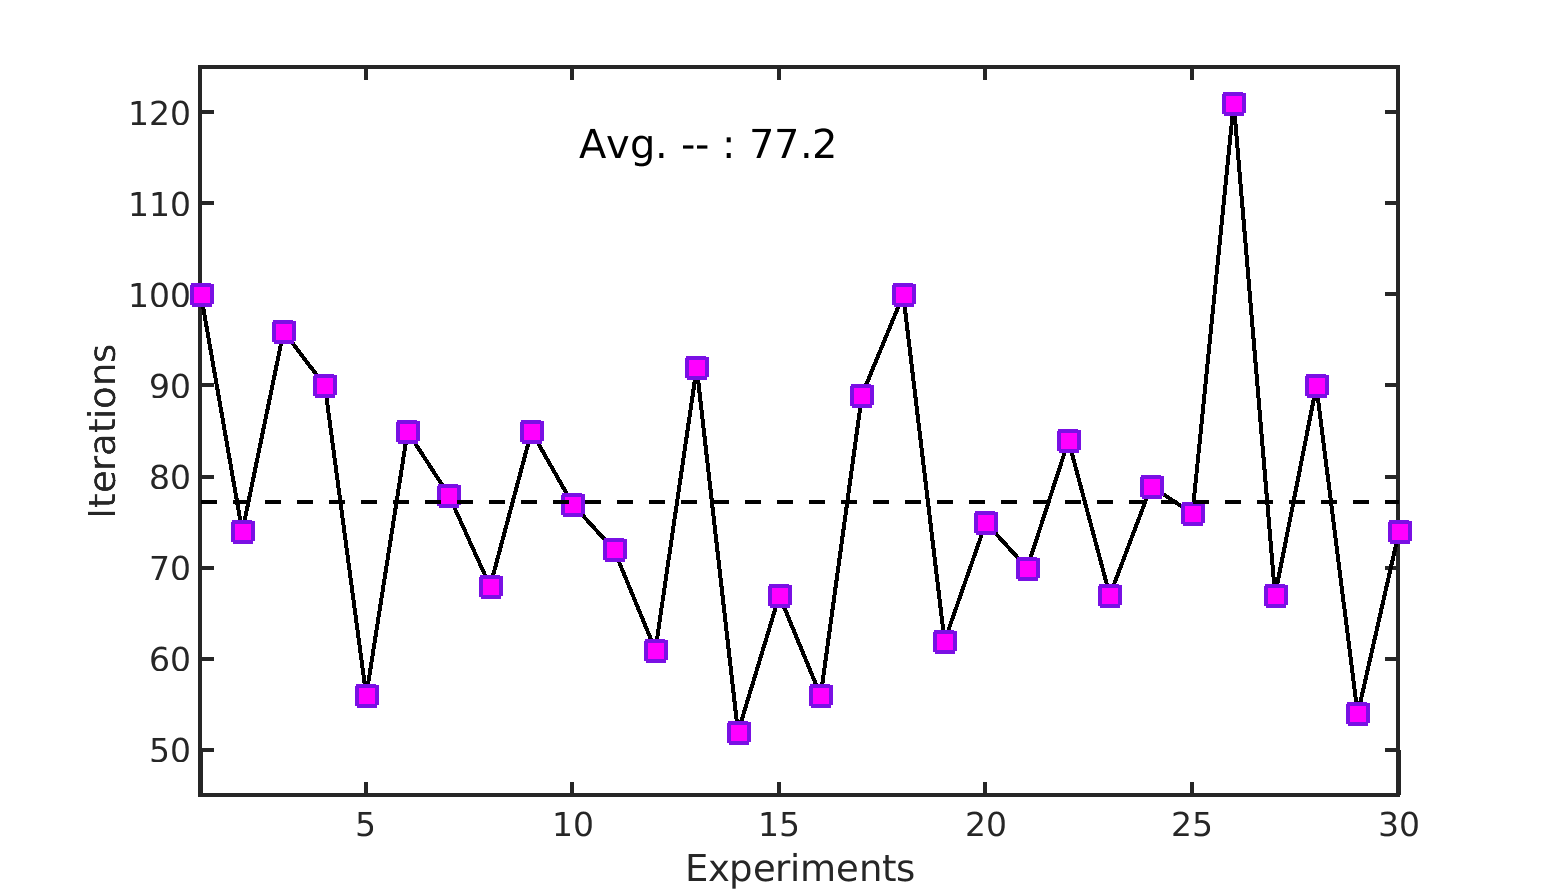
\includegraphics[scale=0.2]{../figures/gauss10Drandr0_1.png}
%      \caption{
%      The required iteration steps of the 
%      HiCS for the Gaussian function
%      \eqref{eqn:exp1} in $30$ runs with randomly generated start points
%      in the space $[-1, 1]^{10}$, and $\rho=0.1$. 
%      The flat dashed line shows the average.} 
%      \label{fig:exp1:randInitr0_1}
%\end{figure}


In the following, we apply the adaptive HiCS to $1000$-dimensional
Gaussian function. The initial value is randomly generated in
domain $[-1000,1000]^{1000}$, the initial search radius $\rho_0 = 2.0$,
and the regulator $\eta=(\sqrt{5}-1)/2$. 
Fig.\,\ref{fig:gauss:1000D} presents the iteration process.
The left image in Fig.\,\ref{fig:gauss:1000D} gives
the difference between $f(x_k)$ and $f(0)=-20$. 
The right one in Fig.\,\ref{fig:gauss:1000D} 
plots the changes of search radius $\rho$ and $\ell^2$-distance between
the iterator and the global minimizer $x^*=0$, where $\|x\|_{\ell^2}=\left(
(\sum_{i=1}^d x_i^2) / d\right)^{1/2}$.
From these results, it can be found that the HiCS is convergent
for each $\rho$. Based on the iteration, the adaptive HiCS 
can approximate the global minimum by decreasing the search radius $\rho$. 
Meanwhile, during the iteration, the global minimizer is always in the
search neighbourhood. 
\begin{figure}[!htbp]
	\begin{minipage}[b]{0.5\linewidth}
	\centering{
	  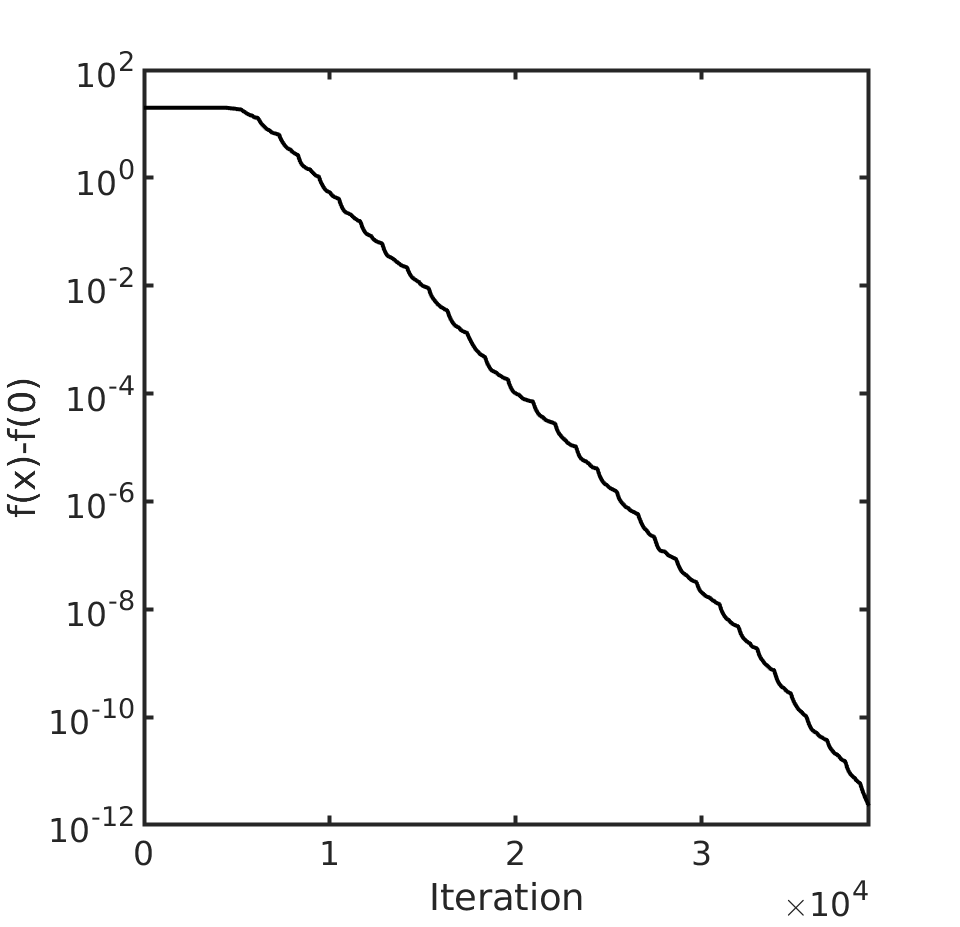
\includegraphics[scale=0.25]{../figures/gauss1000D.png}
	  }
%    \centerline{(a) }
	\end{minipage}
	\begin{minipage}[b]{0.5\linewidth}
	\centering{
	  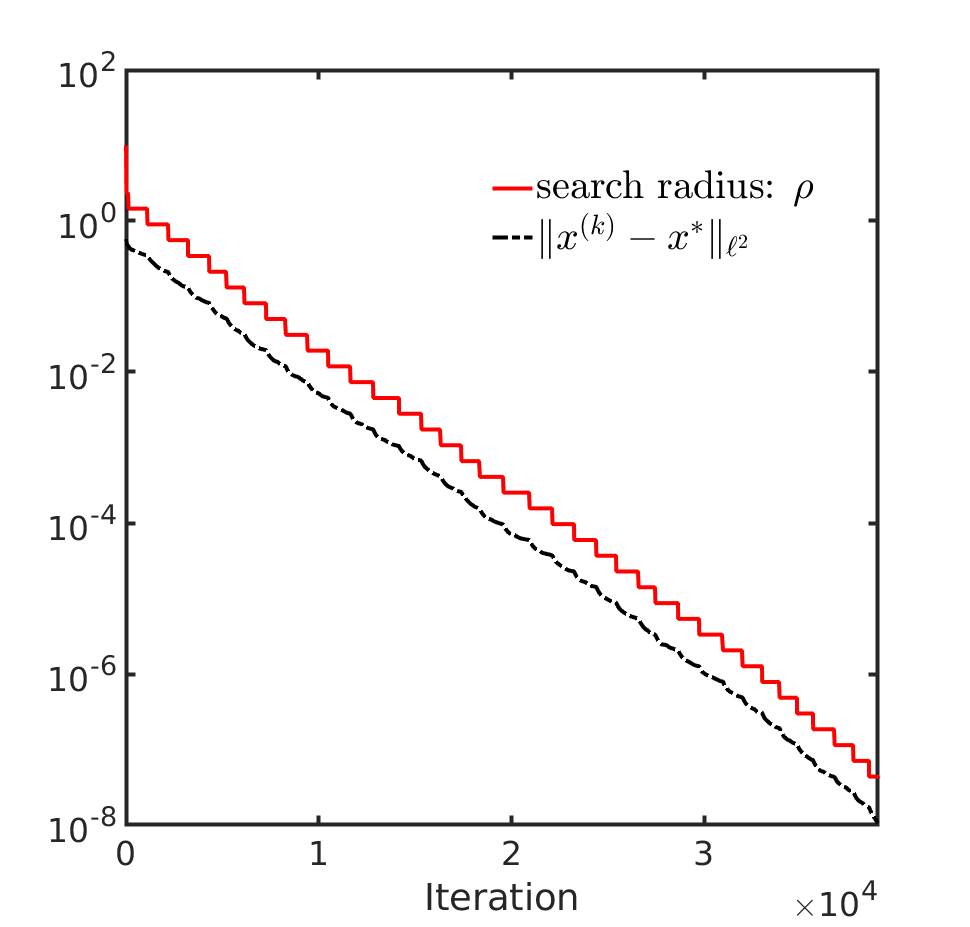
\includegraphics[scale=0.25]{../figures/gauss1000D_dist.png}
	  }
%    \centerline{(b) }
	\end{minipage}
	  \caption{The iteration process of the adaptive HiCS to 1000-dimensional Gaussian function. 
	  Start point is randomly generated in the space $[-1000,
	  1000]^{1000}$, $\rho=2.0$ and the regulator
	  $\eta=(\sqrt{5}-1)/2$. The left plot is the energy
	  difference, and the right one is the search radius and 
	  the $\ell^2$ distance between the current iterator and the
	  global minimizer $x^*=0$.
	  } 
	  \label{fig:gauss:1000D}
\end{figure}

\subsection{The multimodal problems: Ackley and Arwhead functions}
\label{subsec:minmulit}

The second objective function is the Ackley
function\,\cite{stacey2003particle, dieterich2012empirical} which is a widely used 
benchmark function for testing optimization algorithms.
The expression of the Ackley function is
\begin{align}
	f(x) =
	-20\cdot\exp\Bigg(-\frac{1}{5}\cdot\sqrt{\frac{1}{d}\sum_{i=1}^d
	x_i^2}\Bigg)-
	\exp\Bigg(\frac{1}{d}\sum_{i=1}^d \cos(2\pi x_i)\Bigg)+20+e,
	\label{eqn:ackley}
\end{align}
where $d$ is the spatial dimension.
Ackley function has many local minima and a unique global
minimizer of $0$ with $f(0)=0$, which poses a risk for
optimization algorithms to be trapped into one of local
minima, such as the traditional hill-climbing method\,\cite{back1996evolutionary}.
Our previous results have shown that the HiCS can capture
different local minimizer and the global minimizer for 2-dimensional Ackley
function through the choice of different $\rho$\,\cite{huang2017hill}.
In this subsection, we will apply the improved HiCS, the Algorithm \ref{alg:AHiCS},
to higher dimensional Ackley function. 
In the following simulation, the regulator
$\eta=(\sqrt{5}-1)/2$.

\begin{table}[!hbpt]
\caption{
The successful number $N_s$ of capturing the global minimizer for
each different initial search radius $\rho_0$ when applying the
adaptive HiCS ($\eta=(\sqrt{5}-1)/2$) to $100$-dimensional Ackley function from $100$ numerical experiments. 
The initial values are randomly generated in $[-10,10]^{100}$.
}
\label{tab:ackley100D:AHiCS}
\begin{center}
\begin{tabular}{|c|c|c|c|c|c|c|c|c|c|c|}
 \hline
  $\rho_0$  & 2.0 & 1.8 & 1.6 & 1.4 & 1.2 & 1.0 & 0.8 & 0.6 & 0.4 & 0.2 
 \\\hline
  $N_s$     & 98  & 99  & 97  & 73  & 93  & 100 & 99  & 84  & 76 & 57 
\\\hline \hline
 $\rho_0$ & 0.1 & 0.09 & 0.08 & 0.07 & 0.06 & 0.05 & 0.04 & 0.03& 0.02 & 0.01
 \\\hline
  $N_s$& 75 & 79 & 72 & 69 & 84 &86 & 52 & 0 & 0 & 0
\\ \hline
\end{tabular}
\end{center}
\end{table}
We first take $100$-dimensional Ackley function as an example to
test the performance of our proposed algorithm for finding minimizers. 
We run the adaptive HiCS 100 times for different initial
search radius $\rho_0$ from $0.01$ to $2.0$.
The start points are all randomly generated in $[-10,10]^{100}$.
The convergent criterion is the search radius smaller than $10^{-10}$.
Tab.\,\ref{tab:ackley100D:AHiCS} gives the successful number
$N_s$ of capturing the global minimizer with different $\rho_0$.  
When the algorithm is successful, the distance between the
convergent SMP and the global minimizer is smaller than the
search radius $\rho < 10^{-10}$.
From these results, it is easy to find that our method can
approximate the global minimizer. 
The value of $\rho_0$ heavily affects the probability of
obtaining the global minimizer. 
When $\rho_0 > 0.04$, the adaptive HiCS can find the global
minimizer with high probability. 
When $\rho_0$ is about $0.04$, 
the successful probability is falling quickly to about $50\%$. 
As $\rho_0$ decreases to smaller than $0.03$, the HiCS could hardly
find the global minimizer.
Besides, it should be pointed out that these so-called unsuccessful
experiments have obtained other local minimizers. 


We continue to apply the adaptive HiCS to $2500$-dimensional
Ackley function. The initial search radius is $\rho_0=3.5$, and
the initial position is generated randomly in $[-10,10]^{2500}$. 
The iteration process is presented in Fig.\,\ref{fig:ackley2500D:AHiCS}. 
For such a high dimensional optimization problem, the iteration
behavior is similar to previous numerical experiments. 
\Note{
When $\rho=3.5$, the HiCS costs $90$ steps to achieve convergence.}
By further shrinking search radius, the adaptive HiCS can
capture global minimizer. As one can see from 
Fig\,\ref{fig:ackley2500D:AHiCS}, the global minimizer always
locates in the search neighbourhood in this case. 
It demonstrates that the HiCS has the capacity of hupping the
local basin to obtain a neighborhood of the global minimizer for such a high
dimensional problem.
\begin{figure}[!htbp] 
	\centering
	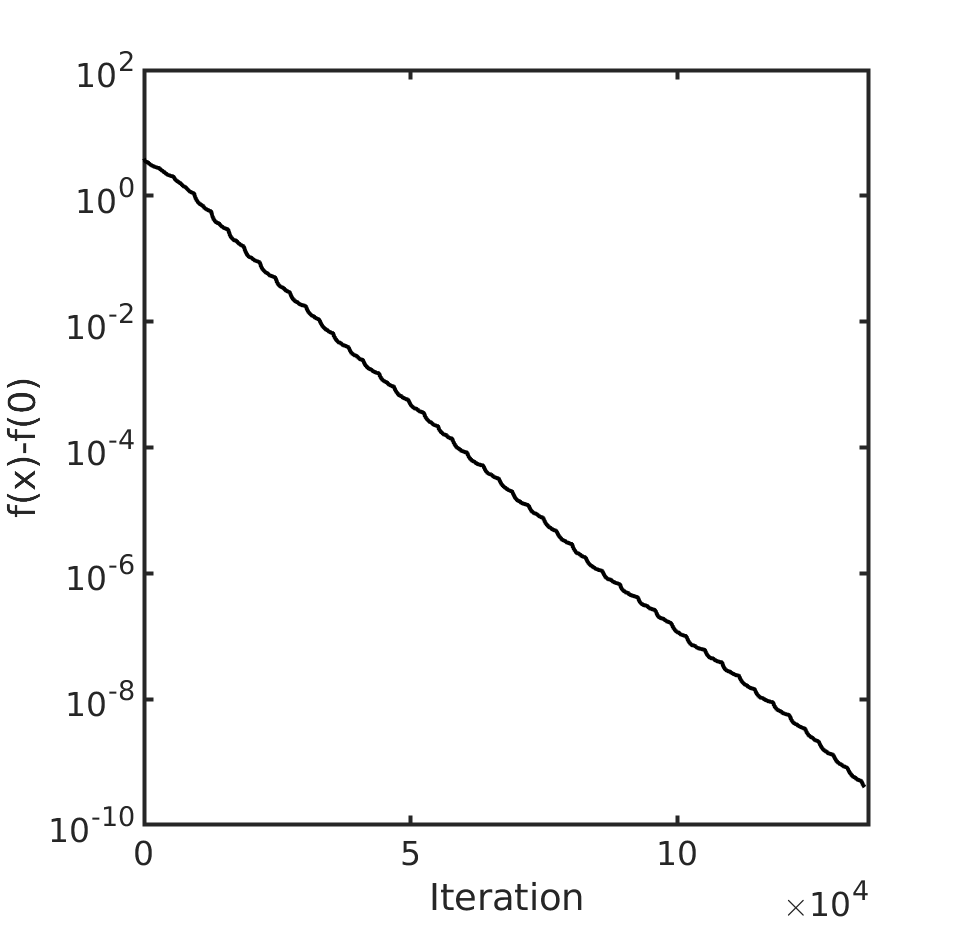
\includegraphics[scale=0.25]{../figures/ackley2500D.png}
	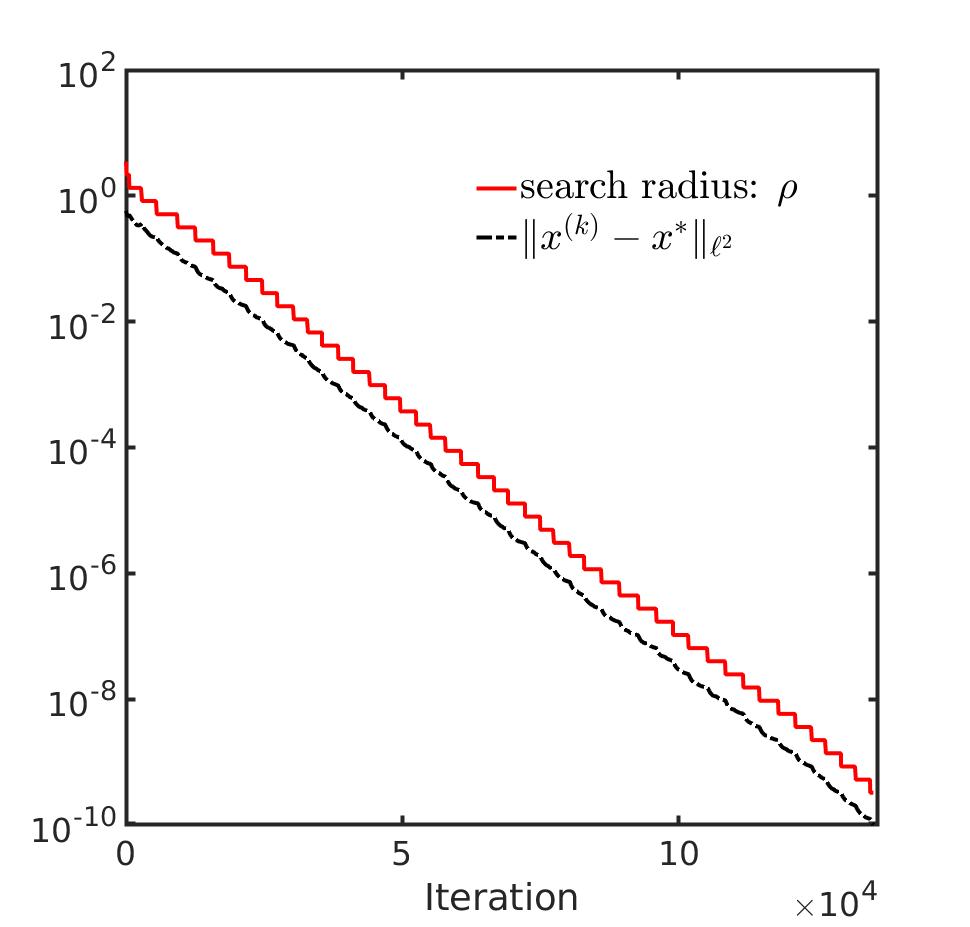
\includegraphics[scale=0.25]{../figures/ackley2500D_dist.png}
	  \caption{The iteration process of the adaptive HiCS to 2500
	  dimensional Ackley function with initial search
	  radius $\rho_0=3.5$. Start point is randomly generated in the
	  space $[-10, 10]^{2500}$. } 
	\label{fig:ackley2500D:AHiCS}
\end{figure}

The last benchmark example is the Arwhead function, which has been
also used by Powell to test the NEWUOA derivative-free
method\,\cite{powell2006newuoa, powell2008developments}. The expression of the Arwhead function is
\begin{align}
	f(x) = \sum_{i=1}^{d-1}[(x_i^2+x_d^2)^2 - 4 x_i +3].
	\label{}
\end{align}
The least value of $f$ is zero, which occurs when the minimizer
$x^*$ take the values $x_j=1$, $j=1,2,\dots,d-1$ and $x_d=0$. 
We directly apply the adaptive HiCS ($\eta=0.5$) to $1000$-dimensional Arwhead function.
The starting vector is given by $x_j^{(0)}=1$, $j=1,2,\dots,d$, as
Powell done in Ref.\,\cite{powell2006newuoa}.
The initial search radius $\rho_0=3$ and $\eta=(\sqrt{5}-1)/2$.
\begin{figure}[!htbp]
	\centering
	  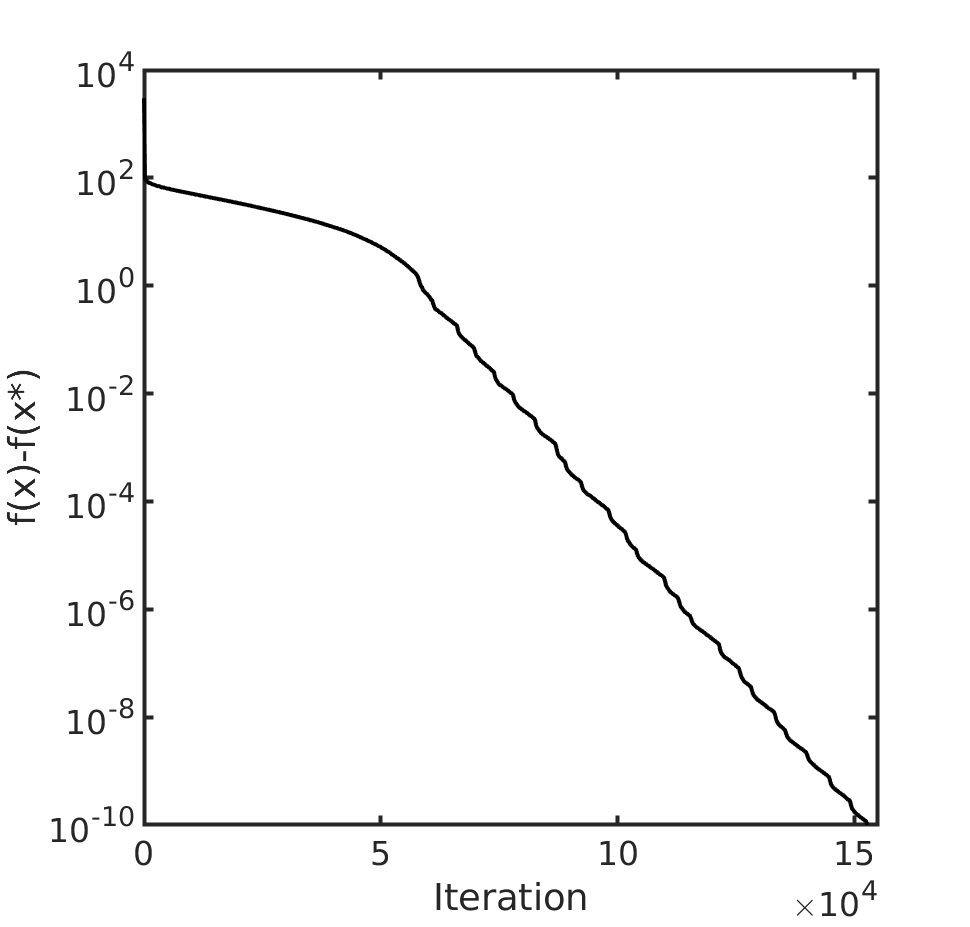
\includegraphics[scale=0.25]{../figures/arwhead1000D.png}
	  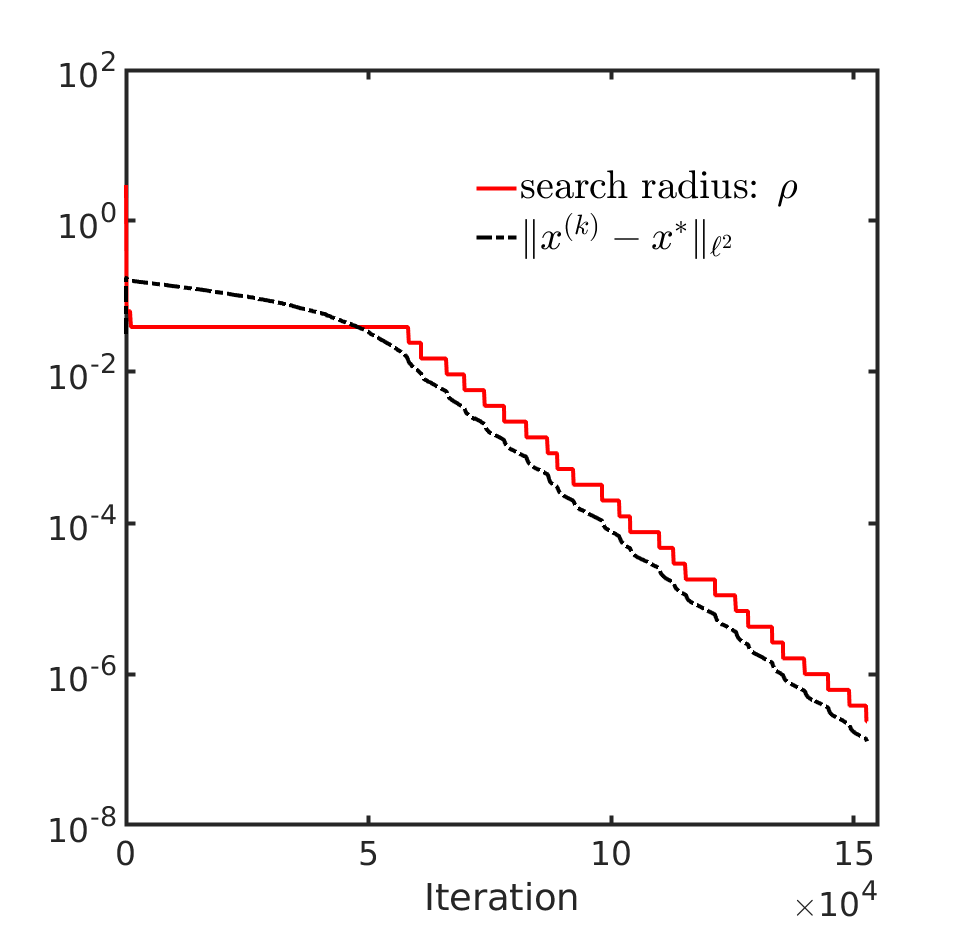
\includegraphics[scale=0.25]{../figures/arwhead1000D_dist.png}
  \caption{The iteration process of the adaptive HiCS 
  ($\eta=(\sqrt{5}-1)/2$) to the $1000$-dimensional Arwhead function.}
	\label{fig:arwhead}
\end{figure}

Fig.\,\ref{fig:arwhead} gives the iteration process of
applying the adaptive HiCS to $1000$-dimensional Arwhead function.
The sequences of function values and iterators approximate the global minimum
and the global minimizer. 
The function value always decreases as the proposed algorithm
indicates. While the distance $\|x^{(k)}-x^*\|_{\ell^2}$
demonstrates more interesting phenomena. In the beginning, the
search radius $\rho$ is larger than the distance, which means the global
minimizer $x^*$ is in the search neighborhood. Then when the distance is
about $1.67\times 10^{-1}$, the $\rho$ is smaller than the
distance, which indicates $x^*$ is not in the search neighborhood. 
It means that the iterator locates in the valley of a local minimizer. 
However, as iteration evolves, the HiCS can jump out of
the local trap well and again contains the global
minimizer in the search region.



\section{Conclusion}
\label{sec:conclusion}

\Note{
In this paper, we introduce a new concept of the SMP to measure the distance between
minimizers and the SMP. We prove that the HiCS converges to a SMP in finite steps. 
To address high dimensional problems, 
we propose an efficient method to discretize subproblem through simplexes in which
the discretization points linearly increase with the spatial dimension.
We apply this HiCS to several benchmarks to examine its performance.
Numerical results demonstrate that the HiCS can efficiently obtain a small
neighbourhood that includes local minimizers, even the global minimizer. 
The obtained results by the HiCS provide a good initial values for other optimization
methods to further find a minimizer. Alternatively, we here shrink the search
radius to directly approximate a minimizer by the HiCS.
}


%\Note{
%Determining a area that contains minimizers is a prerequisite for the
%success of optimization methods.  
%Inspired by the hill-climbing behavior of the blind, we 
%propose the HiCS to find a satisfactory area. The HiCS is easy to implement and has
%only one parameter, the search radius $\rho$, to be adjusted.
%More significantly, we establish a rigorous convergent analysis to guarantee the HiCS
%within finite steps by introducing a new concept of the SMP. 
%To address high dimensional problems, we propose an efficient method
%to discretize subproblem through simplex in which the discretization points linearly increase
%as the spatial dimension. We apply this approach to several benchmarks.
%Numerical results demonstrate that the HiCS can efficiently obtain a neighbourhood
%with $\rho$ that includes local minimizers, even the global minimizer. 
%The obtained results by the HiCS provide a good initial values for other optimization
%methods to further find a minimizer. Alternatively we can shrink the search
%radius $\rho$ to directly approximate a minimizer by the HiCS.
%}


\section*{Acknowledgments}
This work is supported by the National Natural Science Foundation of China (11971410,
11771368) and Project for Hunan National Applied Mathematics Center of Hunan
Provincial Science and Technology Department (2020ZYT003).
KJ is partially supported by the Key Project of the Education Department of 
Hunan Province of China (19A500). 


\begin{thebibliography}{99}

\bibitem{sun2006optimization}
W.~Y.~Sun and Y.~Yuan,
Optimization theory and methods: nonlinear programming,
New York: Springer, 2006.

%\bibitem{conn2000trust}
%A.~R.~Conn, N.~I.~M.~Gould and P.~L.~Toint,
%Trust region methods, Philadelphia: SIAM, 2000.

\bibitem{nocedal2006numerical}
J.~Nocedal and S.~J.~Wright,
Numerical optimization, 
Berlin: Springer-Verlag, 2nd ed., 2006.

\bibitem{conn2009introduction}
A.~R.~Conn, K.~Scheinberg and L.~N.~Vicente,
Introduction to derivative-free optimization,
Philadelphia: SIAM, 2009.

\bibitem{huang2017hill}
{Y.~Huang and K.~Jiang,}
{Hill-climbing algorithm with a stick for unconstrained optimization problems},
{Adv. Appl. Math. Mech.},
2017, 9: 307--323.

\bibitem{stacey2003particle}
  {A.~Stacey, M.~Jancic, and I.~Grundy},
  {Particle swarm optimization with mutation},
  In \textit{Proceedings of the Congress on Evolutionary Computation}, pages
1425–1430, Camberra, Australia, 2003. IEEE Press.


  {The 2003 Congress on Evolutionary Computation, CEC03},
  2003, 2: 1425--1430.

\bibitem{dieterich2012empirical}
J.~M.~Dieterich and B.~Hartke, 
Empirical review of standard benchmark functions using evolutionary global optimization,
{Appl. Math.} 2012, 3: 1552--1564.

\bibitem{back1996evolutionary}
T.~B{\"a}ck, 
Evolutionary algorithms in theory and practice: evolution
  strategies, evolutionary programming, genetic algorithms,
Oxford University Press, 1996.

\bibitem{powell2006newuoa}
M.~J.~D.~Powell,
The NEWUOA software for unconstrained optimization without derivative, in
Large-Scale Nonlinear Optimization , eds. G.~Di~Pillo
and M.~Roma, Springer (New York), 2006, 255--297.

\bibitem{powell2008developments}
M.~J.~D.~Powell,
Developments of NEWUOA for minimization without derivatives,
IMA J. Numer. Anal.,
2008, 28: 649--664.


%%\bibitem{rios2013derivative}
%%L.~M.~Rios and N.~V.~Sahinidis,
%%Derivative-free optimization: a review of algorithms and comparison
%%  of software implementations.
%%{J. Global Optim.}, 2013, 56: 1247--1293.
%%
%\bibitem{powell2000uobyqa}
%M.~J.~D.~Powell, UOBYQA: unconstrained optimization by quadratic
%approximation, Technical Report DAMTP NA2000/14, CMS, University
%of Cambridge, 2000.
%
%\bibitem{powell2002trust}
%M.~J.~D.~Powell, On trust region methods for unconstrained
%minimization without derivatives, Technical Report DAMTP
%NA2002/NA02, CMS, University of Cambridge, February 2002.
%
%%\bibitem{wu2009heuristic}
%%T.~Wu, Y.~Yang, L.~Sun, and H.~Shao, A heuristic
%%iterated-subspace minimization method with pattern search for
%%unconstrained optimization, 
%%Comput. Math. Appl., 2009, 58: 2051-2059.
%%
%\bibitem{zhang2014sobolev}
%Z.~Zhang, Sobolev seminorm of quadratic functions with
%applications to derivative-free optimization, Math. Program.,
%2014, 146: 77-96.
%
%\bibitem{michalewicz2004how}
%Z. Michalewicz and D. B. Fogel, How to solve it: modern
%heuristics, Springer, 2004.
%
%%\bibitem{lecun2015deep}
%%Y.~LeCun, Bengio, Y.~Hinton, G.~Hinton, Deep learning, Nature,
%%2015, 521: 521-436.
%%
%%\bibitem{hooke1961direct}
%%R.~Hooke and T.~A.~Jeeves,
%%``Direct search'' solution of numerical and statistical problems,
%%{J. ACM}, 1961, 8: 212--229.
%%
%\bibitem{lewis2000direct}
%R.~M.~Lewis, V.~Torczon and M.~W.~Trosset,
%Direct search methods: then and now,
%{J. Comput. Appl. Math.},
%2000, 124: 191--207.
%
%\bibitem{nelder1965simplex}
%J.~A.~Nelder and R.~Mead,
%A simplex method for function minimization,
%{Comput. J.}, 1965, 7: 308--313.
%
%\bibitem{torczon1997convergence}
%V.~Torczon,
%On the convergence of pattern search algorithms,
%{SIAM J. Optim.}, 1997, 7: 1--25.
%
\bibitem{kolda2003optimization}
T.~G.~Kolda, R.~W.~Lewis and V.~Torczon,
Optimization by direct search: new perspectives on some classical
and modern methods,
{SIAM Rev.}, 2003, 45: 385--482.

%\bibitem{dennis1991direct}
%J.~E.~Jr Dennis and V.~Torczon,
%Direct search methods on parallel machines,
%{SIAM J. Optim.}, 1991, 1: 448--474.
%
%\bibitem{gratton2015direct} 
%S.~Gratton, C.~W.~Royer, L.~N.~Vicente, Z.~Zhang, Direct search
%based on probabilistic descent, SIAM J.~Optim., 
%2015, 25:1515-1541.
%
%\bibitem{russell2010artificial} 
%S.~J.~Russell and P.~Norvig,  Artificial intelligence: a modern
%approach, 3rd ed., Prentice Hall, 2010.
%
%\bibitem{dennis1987optimization}
%J.~E.~Jr Dennis and D.~J.~Woods,
%Optimization on microcomputers: The Nelder-Mead simplex algorithm.
%In: New computing environments: microcomputers in large-scale
%computing, A.~Wouk ed., Philadelphia: SIAM, 1987.
%
%%\bibitem{lukvsan2010modified}
%%L.~Luk{\v{s}}an, C.~Matonoha, J.~Vlcek,
%%Modified CUTE problems for sparse unconstrained optimization,
%%Techical Report,
%%2010, 1081.
%
%%\bibitem{algopy}
%%https://pythonhosted.org/algopy/index.html
%
%%\bibitem{andrei2008unconstrained}
%%N.~Andrei, 
%%An unconstrained optimization test functions collection,
%%Adv. Model. Optim.,
%%2008, 10: 147--161.


\end{thebibliography}
	
\end{document}
